\documentclass[a4paper, 10pt]{scrartcl}
\usepackage{amsmath}
\usepackage{graphicx}
\usepackage[colorlinks]{hyperref}
\usepackage{typearea}
\typearea{12}
\makeatletter
\newcommand{\figcaption}[1]{\def\@captype{figure}\caption{#1}}
\newcommand{\tblcaption}[1]{\def\@captype{table}\caption{#1}}
\makeatother
\begin{document}

\title{Comparison of 7m-array observations with ACACORR and BLC: CSV-3664 ClusterC}
\author{Seiji Kameno, Jennifer Donovan Meyer, Antonio Hales}
% \date{\today}
\maketitle
\begin{abstract}
Here are comparison of Band-6 7m-array mosaic observations correlated by the baseline correlator (BLC) and ACA correlator (ACAC).
We have run two ExecBlocks with ACAC and BLC consequently near the transit of the target source ClusterC to minimize the differences in $(u, v)$ coverage.
The results in continuum flux density of the point-like phase calibrator are consistent between two correlators.
For the target source, however, the continuum flux density and line intensities measured with BLC are slightly higher than that with ACAC by $\sim 10$\%.
We consider the difference would be ascribed to different responses to the extended structure of the target source by different position angles of the relatively high sidelobes.
\end{abstract}

\section{Introduction}
CSV-3664 is to verify the consistency of 7m-array executions with both BLC and ACAC. The purpose is to enable contingency in case the ACAC stops working due to hardware problems or decommission.
We have reported the initial comparison results of Band-6 observations in \href{http://www.alma.cl/~skameno/Documents/CSV-3664/}{CSV-3664 report}. There, most of results are consistent between two correlators, except strong emission lines that required renormalization correction.

\begin{figure}[h]
	\centering
	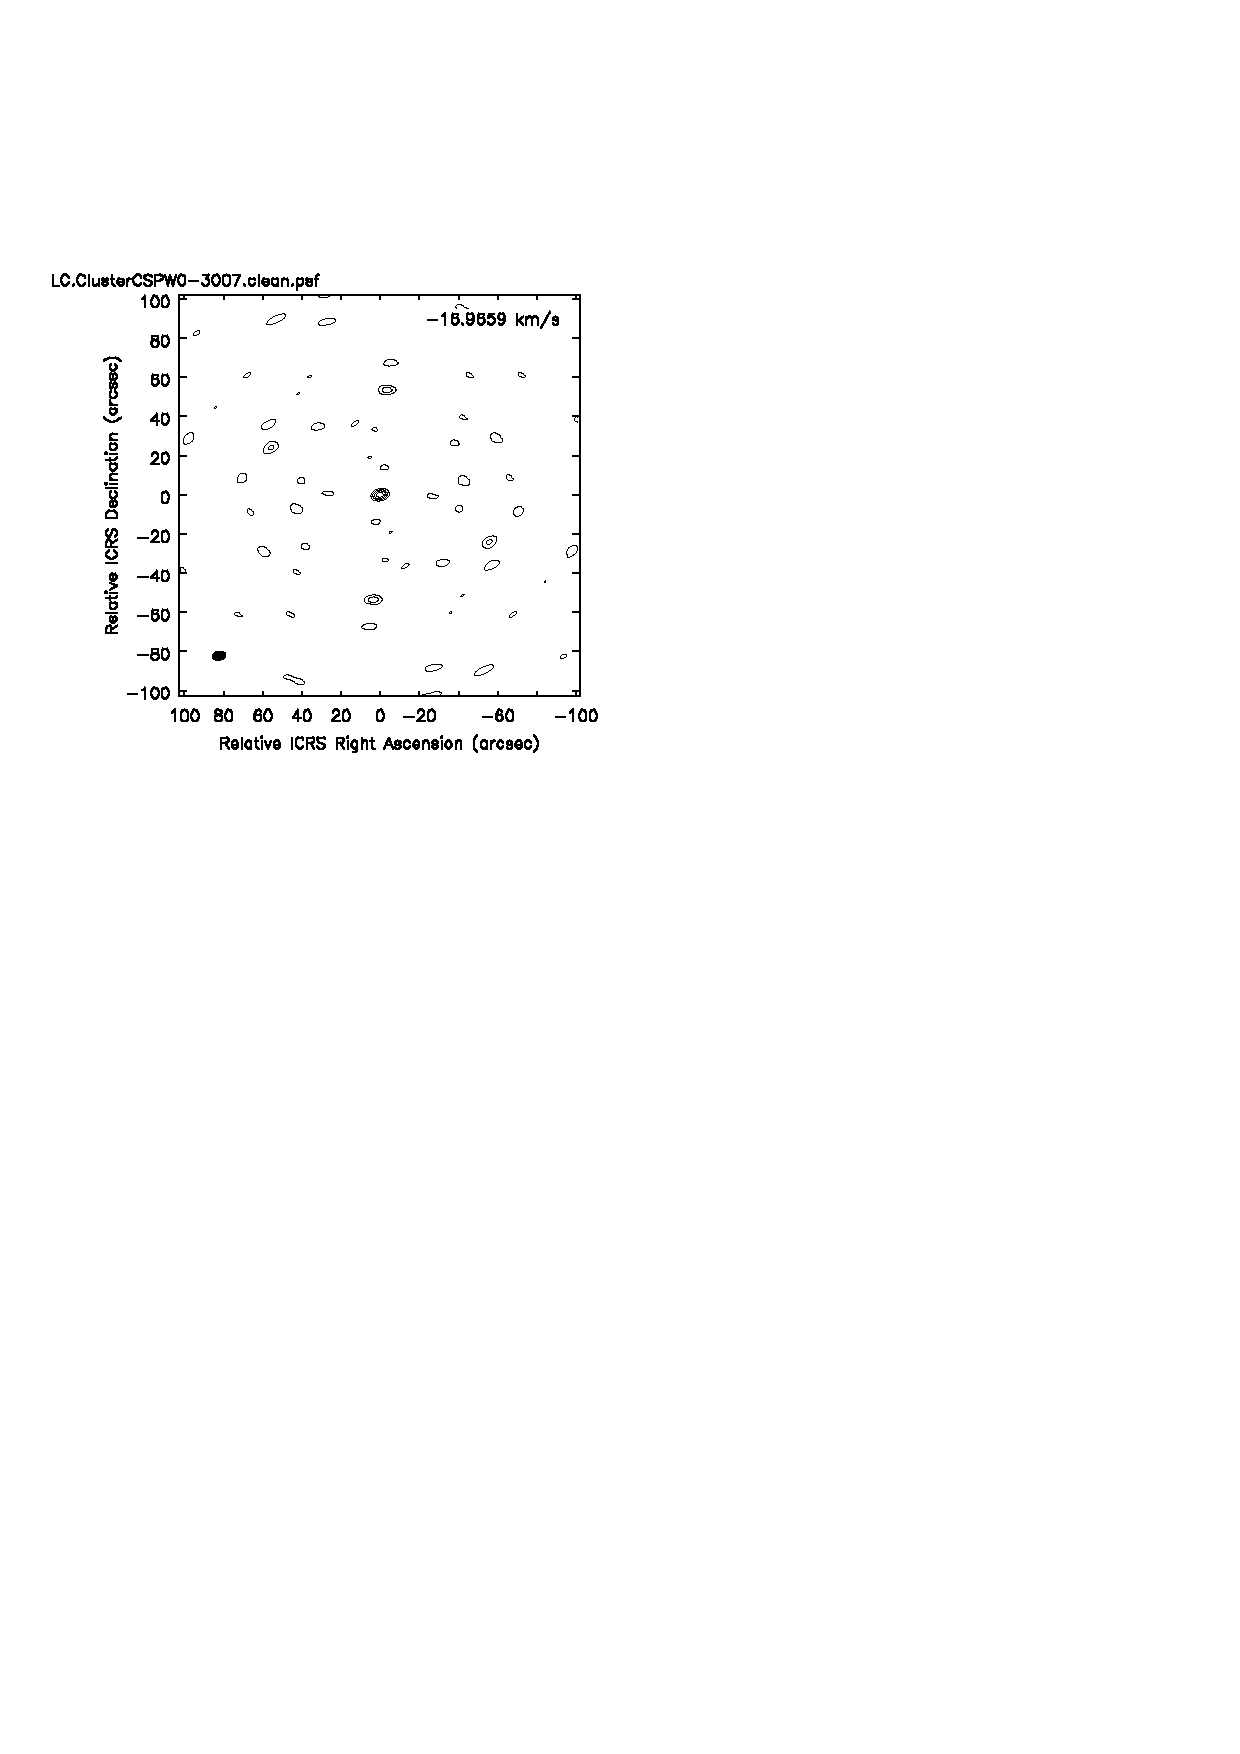
\includegraphics[width=5cm]{BLC-beam.pdf} 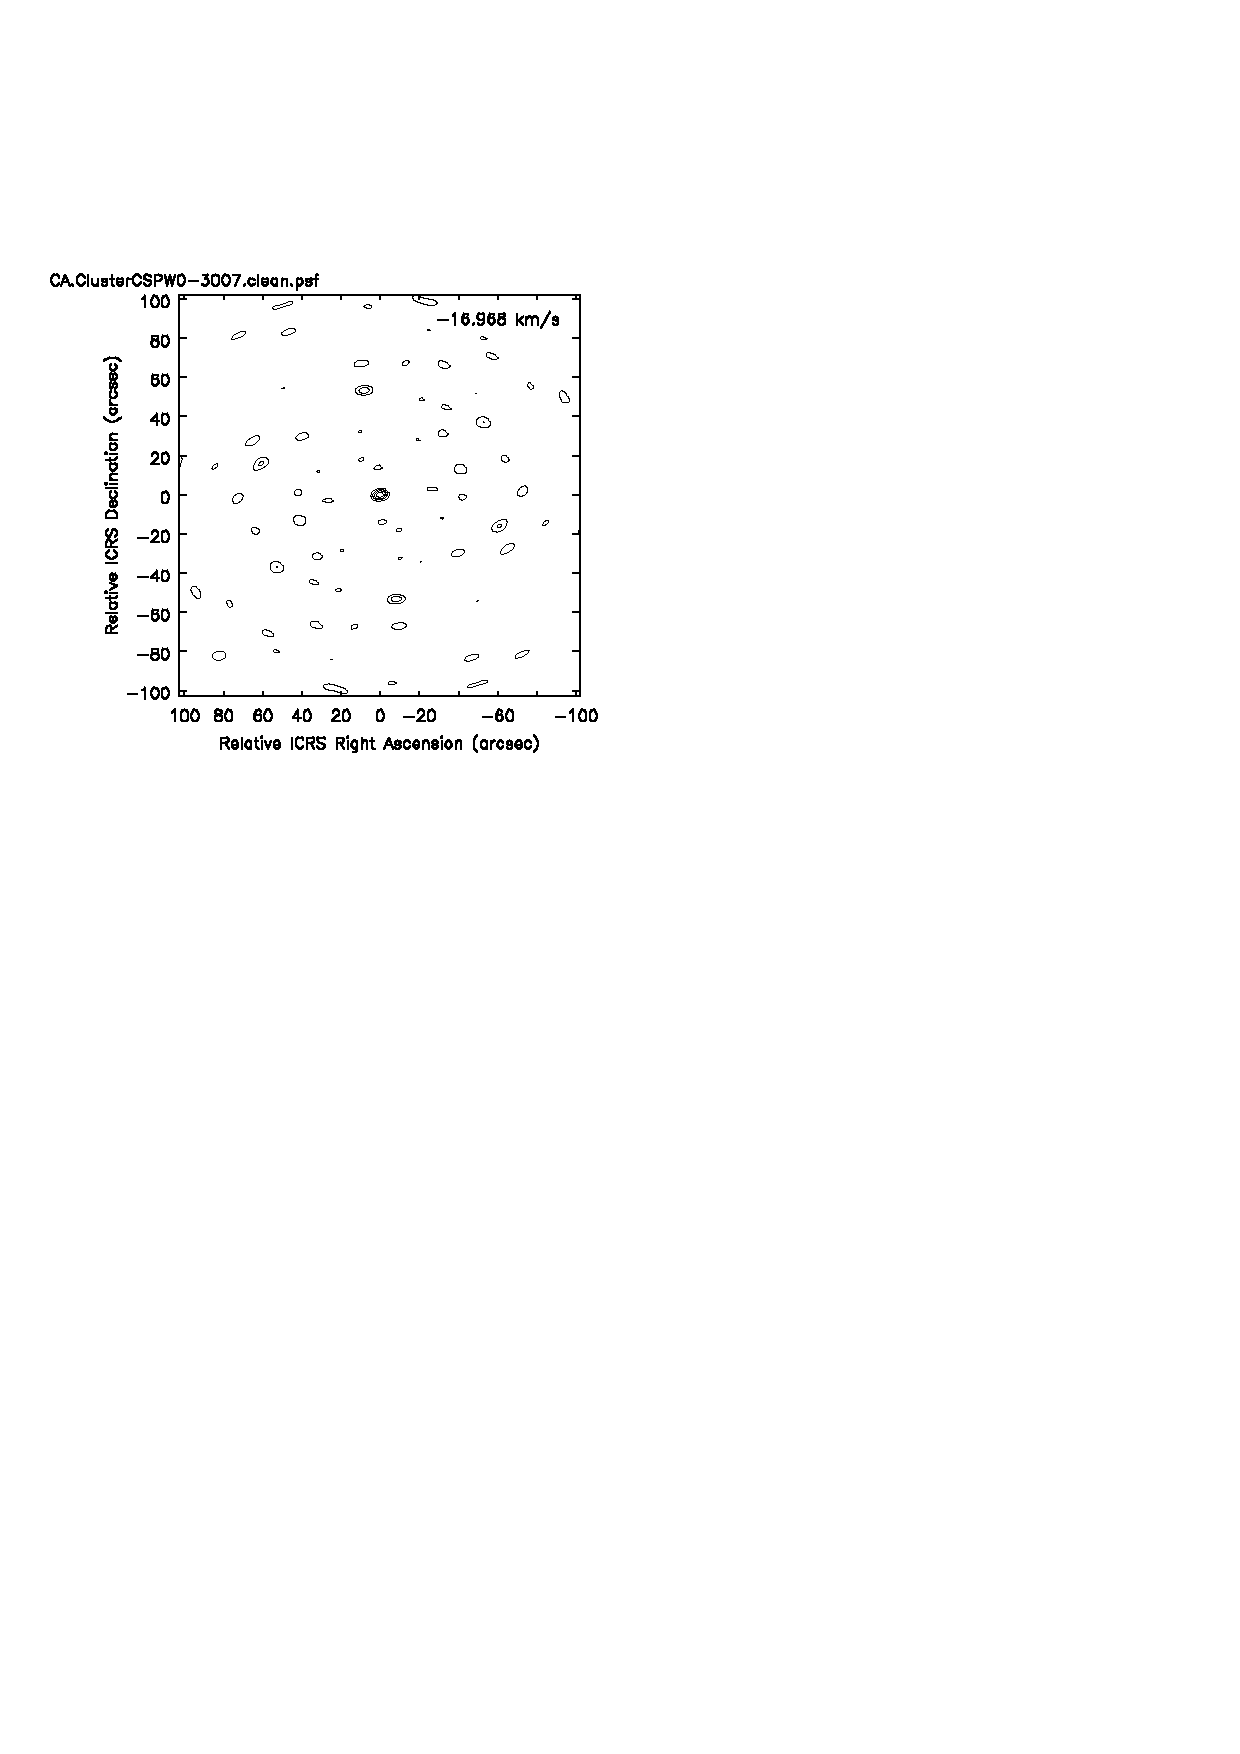
\includegraphics[width=5cm]{ACA-beam.pdf}
	\caption{Synthesized beams of ExecBlocks Xf7fc66/Xac6e with BLC (left) and Xf7fc66/Xb59b with ACAC (right). Contour levels are $-0.2, +0.2, +0.4, +0.6, +0.8$. The maximum sidelobe levels are 0.5381 and 0.5445, while the lowest negative are -0.1608 and -0.1892 for BLC and ACAC, respectively. Because of the difference in HA ranges between two executions, the position angles of the sidelobes are different.}\label{fig:PSF}
\end{figure}


\section{Methods: Science SB executions on 2022-04-25}
We carried out two 7m-array ExecBlocks with BLC and ACAC using the SB in the Project Code E2E6.1.00068.S (copied from 2018.1.01431.S).
Two executions with ACAC and BLC were carried out straddling the transit, to obtain similar $(u,v)$ coverage.
As shown in figure \ref{fig:PSF}, however, the position angles of the sidelobes are different due to difference in HA ranges.

Executions are listed in tables \ref{tab:EBlist}. Two executions with equivalent SBs. Both SBs were generated using the same SG, but one was generated for the BLC and the other for the ACAC.


\begin{table}[h]
\centering
\caption{Execution blocks}
\label{tab:EBlist}
\begin{tabular}{lllll} \hline \hline
Correlator & Date        & EB  uid://A002/   & Start--End (UTC)    & Synthesized beam  \\ \hline 
BLC        & 2022-04-25  & Xf7fc66/Xac6e & 06:13:55 - 07:26:57 & $7^{\prime \prime}.1\times 4^{\prime \prime}.6$ PA$=82^{\circ}.5$ \\
ACAC       & 2022-04-25  & Xf7fc66/Xb59b & 07:34:23 - 08:37:48 & $7^{\prime \prime}.0\times 4^{\prime \prime}.7$ PA$=82^{\circ}.2$ \\ \hline
\end{tabular}
\end{table}

Standard manual data reduction with CASA (version PIPELINE 6.2.1.7) has been carried out to produce image cubes of two targets.
Standard amplitude calibration, bandpass calibration, phase calibration processes were applied.
See the reduction script \href{https://jira.alma.cl/secure/attachment/457290/ClusterC.py}{ClusterC.py}.

For BLC, $T_{\mathrm{sys}}$ spectra are acquired in TDM SPWs which has a coarser spectral resolution than FDM SPWs, while ACAC employs the common spectral setup for both atmCal and interferometry scans.

The SSR selected different flux calibrators, J1427-4206 and J1924-2914, for the ExecBlocks Xf7fc66/Xac6e and Xf7fc66/Xb59b, respectively.
We examined consistency in flux scaling by comparing flux density of the common phase calibrator, J1733-3722, and concluded that the difference in flux scaling is smaller than 0.2\%. See section \ref{subsec:phasecal}.

Note that the reduction procedure does NOT contain non-standaard calibration processes such as renormalization steps.
The flux density of emission lines were up to 3 Jy, which was negligible with respect to the SEFD of $\sim 8000$ Jy.
Thus, skipping renormalization steps won't significantly affect comparison in spectral line profiles.

Common features of executions are listed below.
\footnotesize
\begin{verbatim}
uid://A002/Xf7fc66/Xac6e (BLC)
#Fields: 56
#  ID   Code Name                RA               Decl           Epoch   SrcId      nRows
#  0    none J1427-4206          14:27:56.297561 -42.06.19.43767 ICRS    0        1819480
#  1    none J1745-2900          17:45:40.036065 -29.00.28.16819 ICRS    1         171000
#  2    none J1733-3722          17:33:15.193076 -37.22.32.39955 ICRS    2        1403080
#  3    none ClusterC            17:00:35.000000 -40.33.44.00000 ICRS    3         236880
#  
#  55   none ClusterC            17:00:40.712004 -40.32.38.20755 ICRS    3         133280

uid://A002/Xf7fc66/Xb59b (ACAC)
#Fields: 55
#  ID   Code Name                RA               Decl           Epoch   SrcId      nRows
#  0    none J1924-2914          19:24:51.055956 -29.14.30.12106 ICRS    0        1816800
#  1    none J1733-3722          17:33:15.193076 -37.22.32.39955 ICRS    1        1222320
#  2    none ClusterC            17:00:35.000000 -40.33.44.00000 ICRS    2         228000
#
#  54   none ClusterC            17:00:40.712004 -40.32.38.20755 ICRS    2         110480
\end{verbatim}
* ClusterC covers 53 mosaic fields hollowed out in the list above.

Time ranges of 07:03:25 ~- 07:03:30 and 07:21:15 -- 07:24:10 in uid://A002/Xf7fc66/Xac6e were flagged out because of anomalous visibilities as shown in figure \ref{fig:flagout}.

\begin{figure}[h]
	\centering
	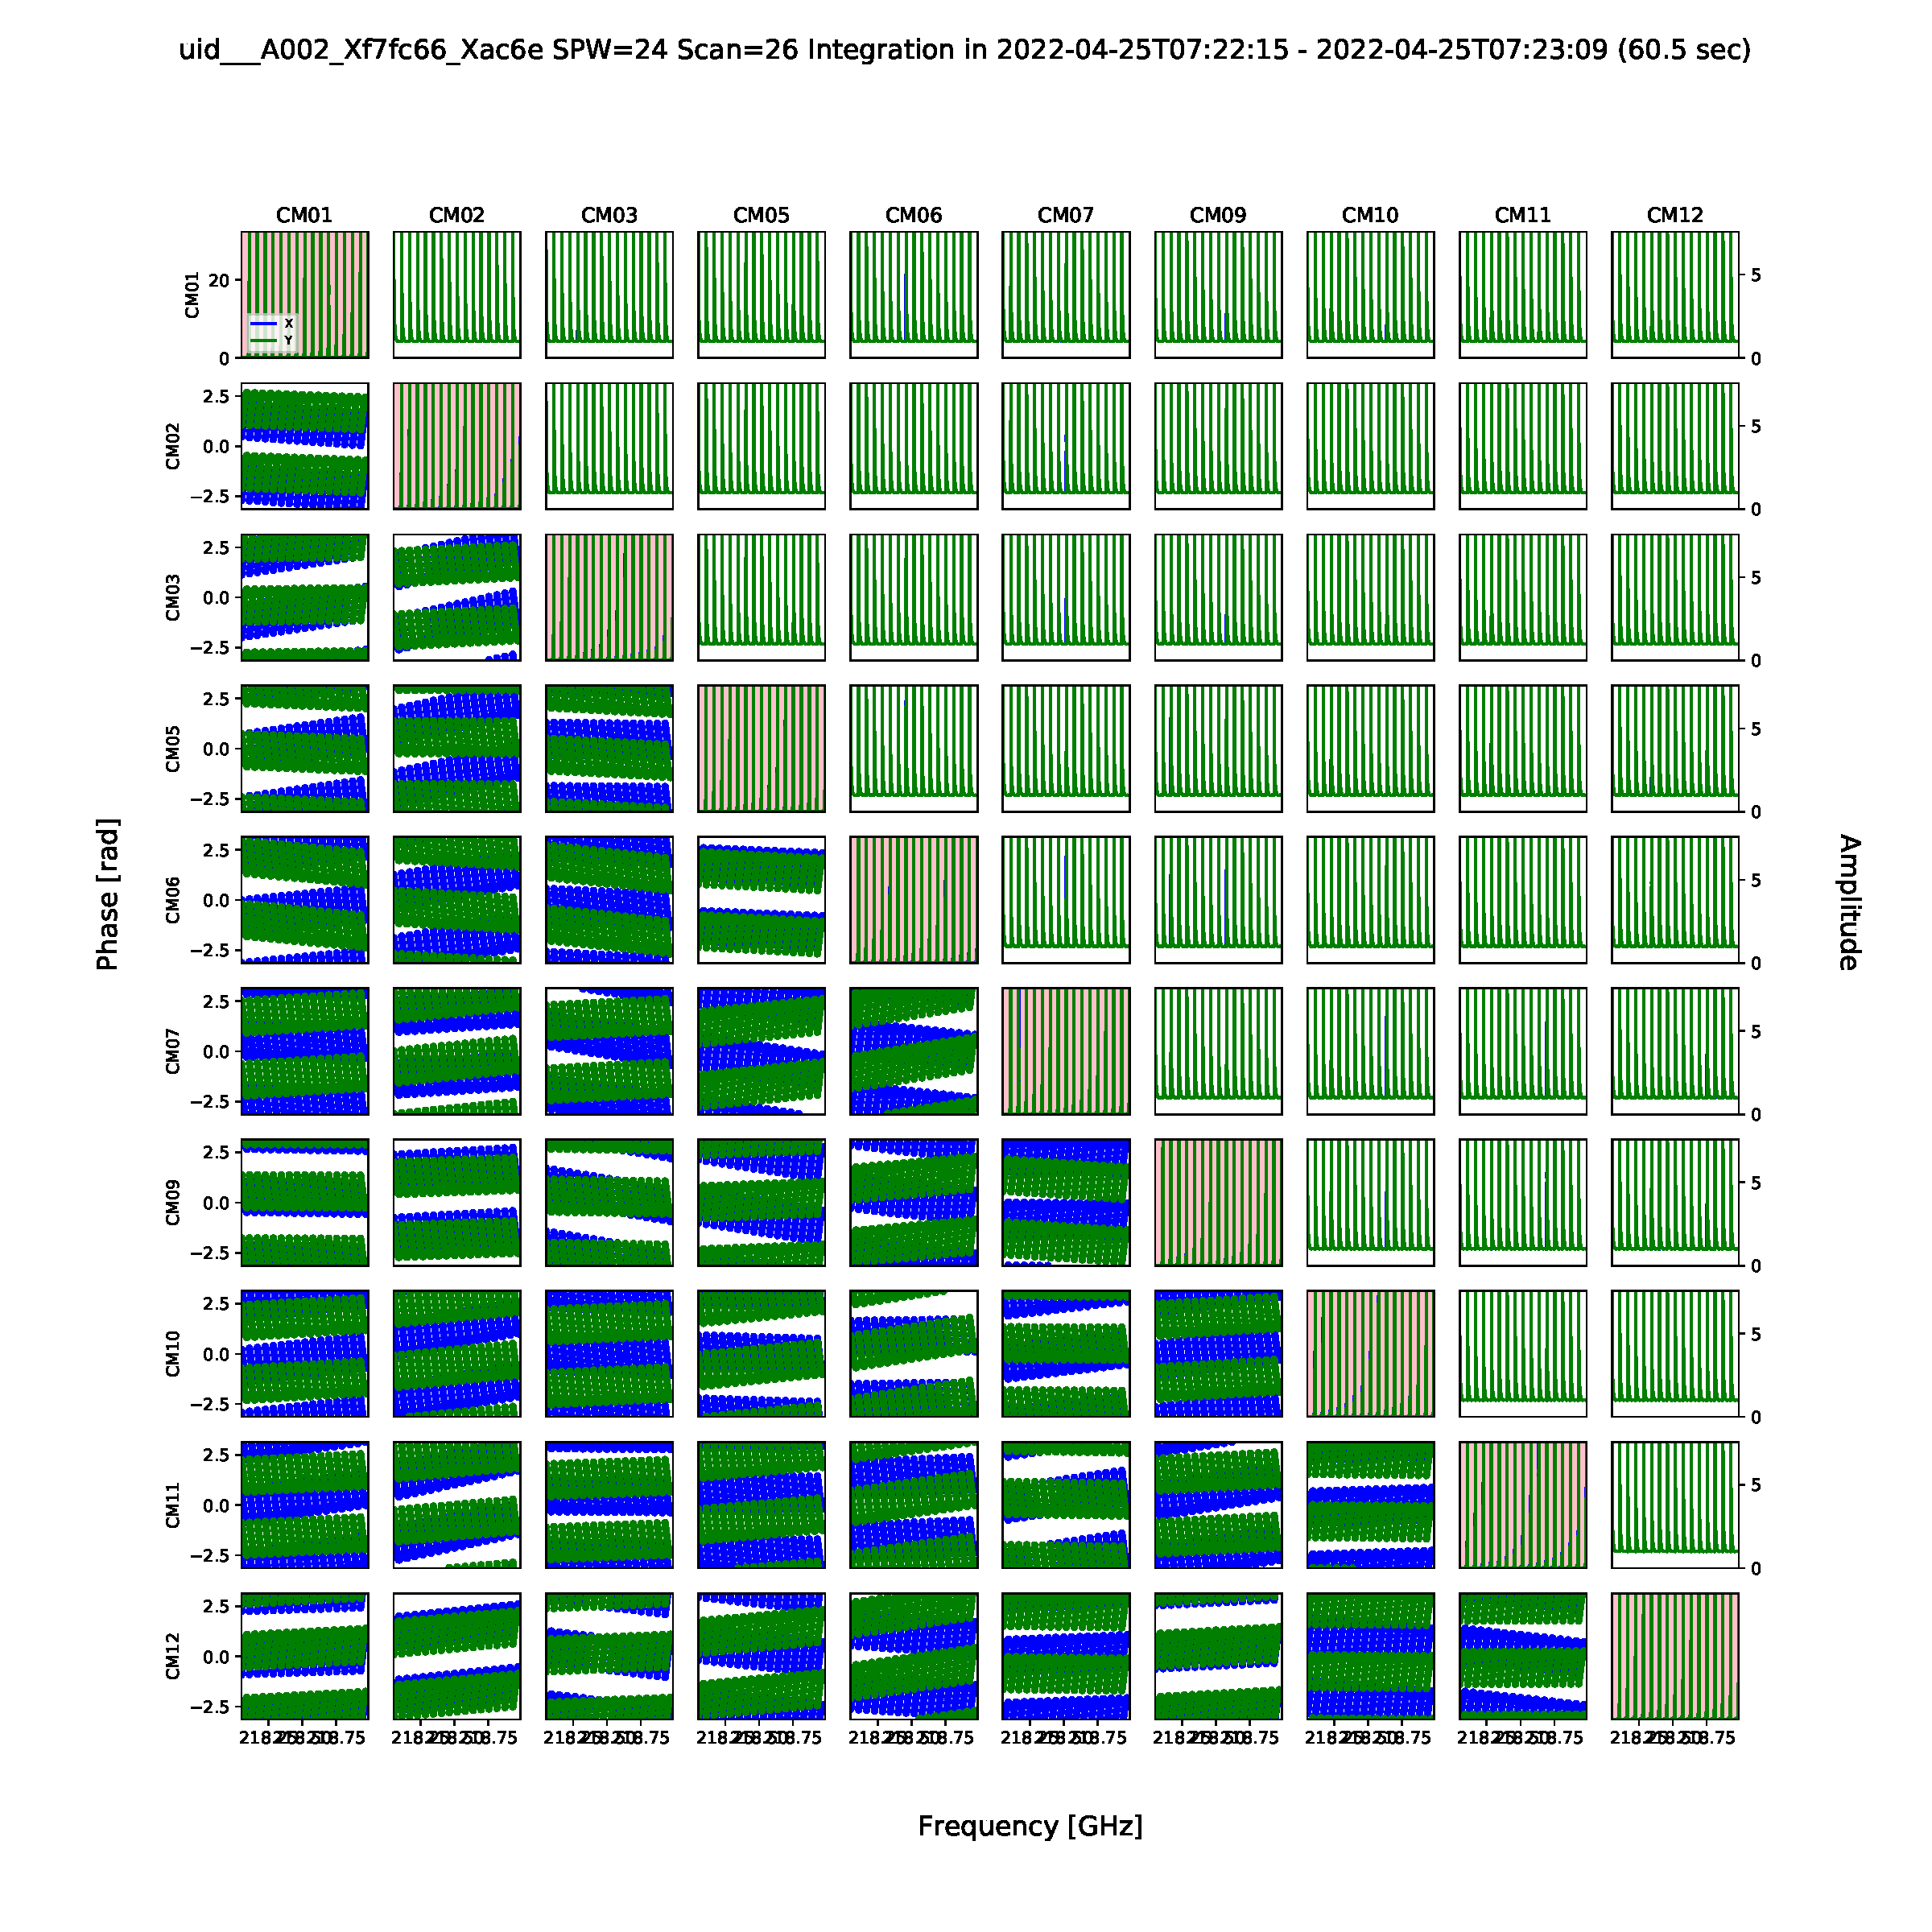
\includegraphics[width=8cm]{PS_uid___A002_Xf7fc66_Xac6e_Scan26_SPW24.pdf}
	\caption{Anomalous cross correlations detected in uid://A002/Xf7fc66/Xac6e. 07:03:25 ~- 07:03:30 and 07:21:15 -- 07:24:10 were flagged out.}\label{fig:flagout}
\end{figure}

Figure \ref{fig:gainamp} show amplitudes and phases of antenna-based gain solutions in bandpass and phase calibration scans. Because of the anomalous visibilities shown in \ref{fig:flagout}, gain solutions in that time range are unrealistic and unused in later processes.

\begin{figure}[h]
	\centering
	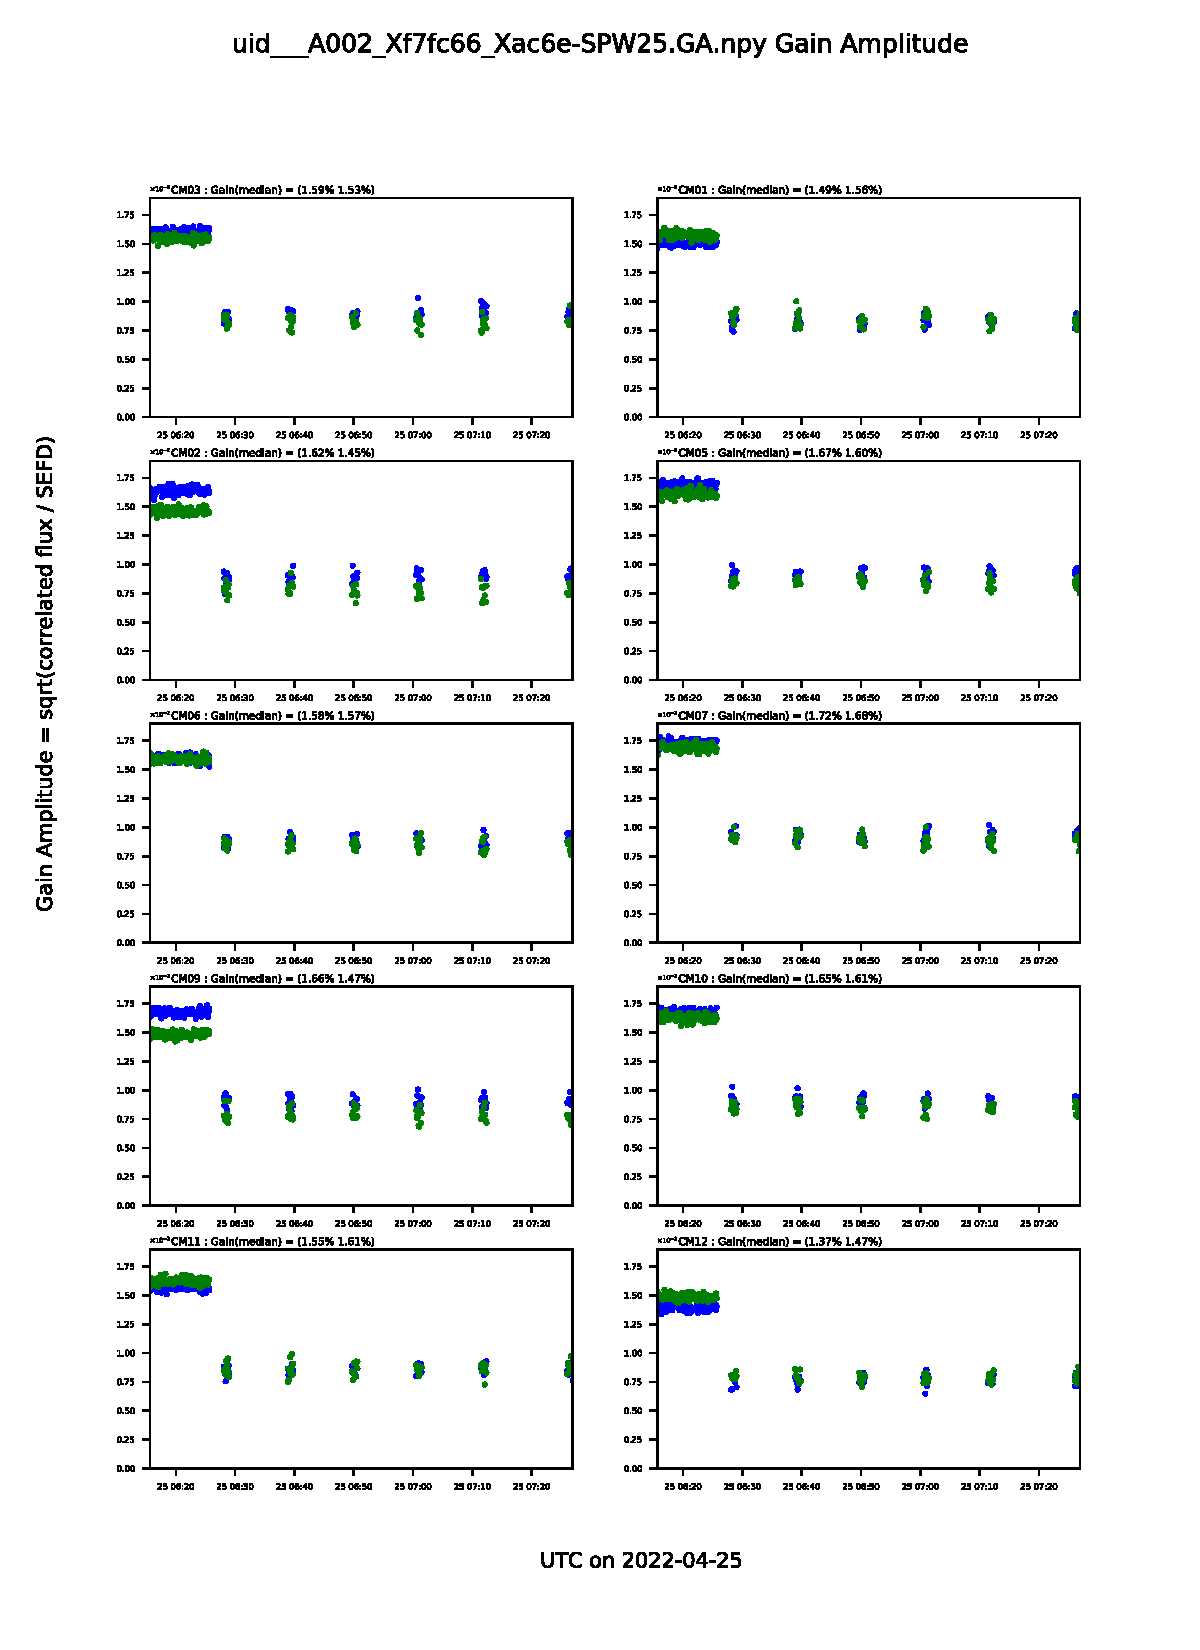
\includegraphics[width=7cm,height=6cm]{GA_uid___A002_Xf7fc66_Xac6e-SPW25-amp.pdf} 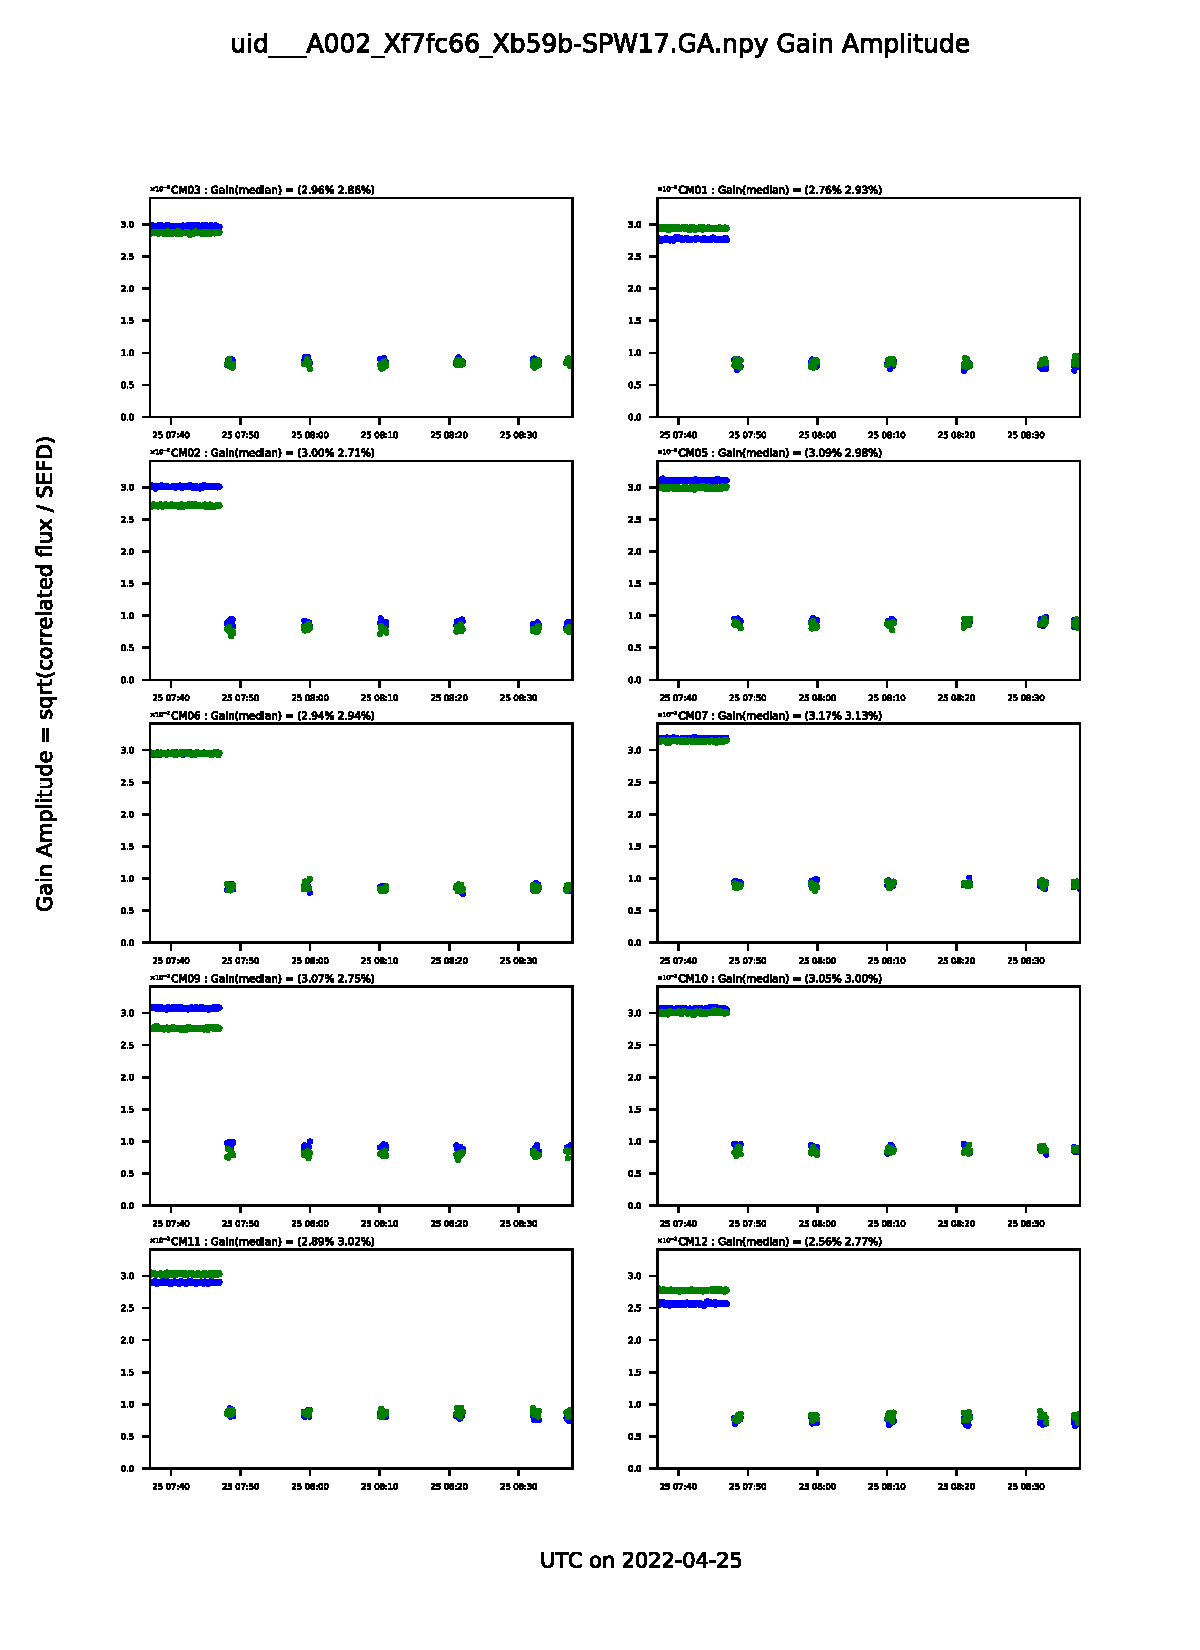
\includegraphics[width=7cm,height=6cm]{GA_uid___A002_Xf7fc66_Xb59b-SPW17-amp.pdf}
	
	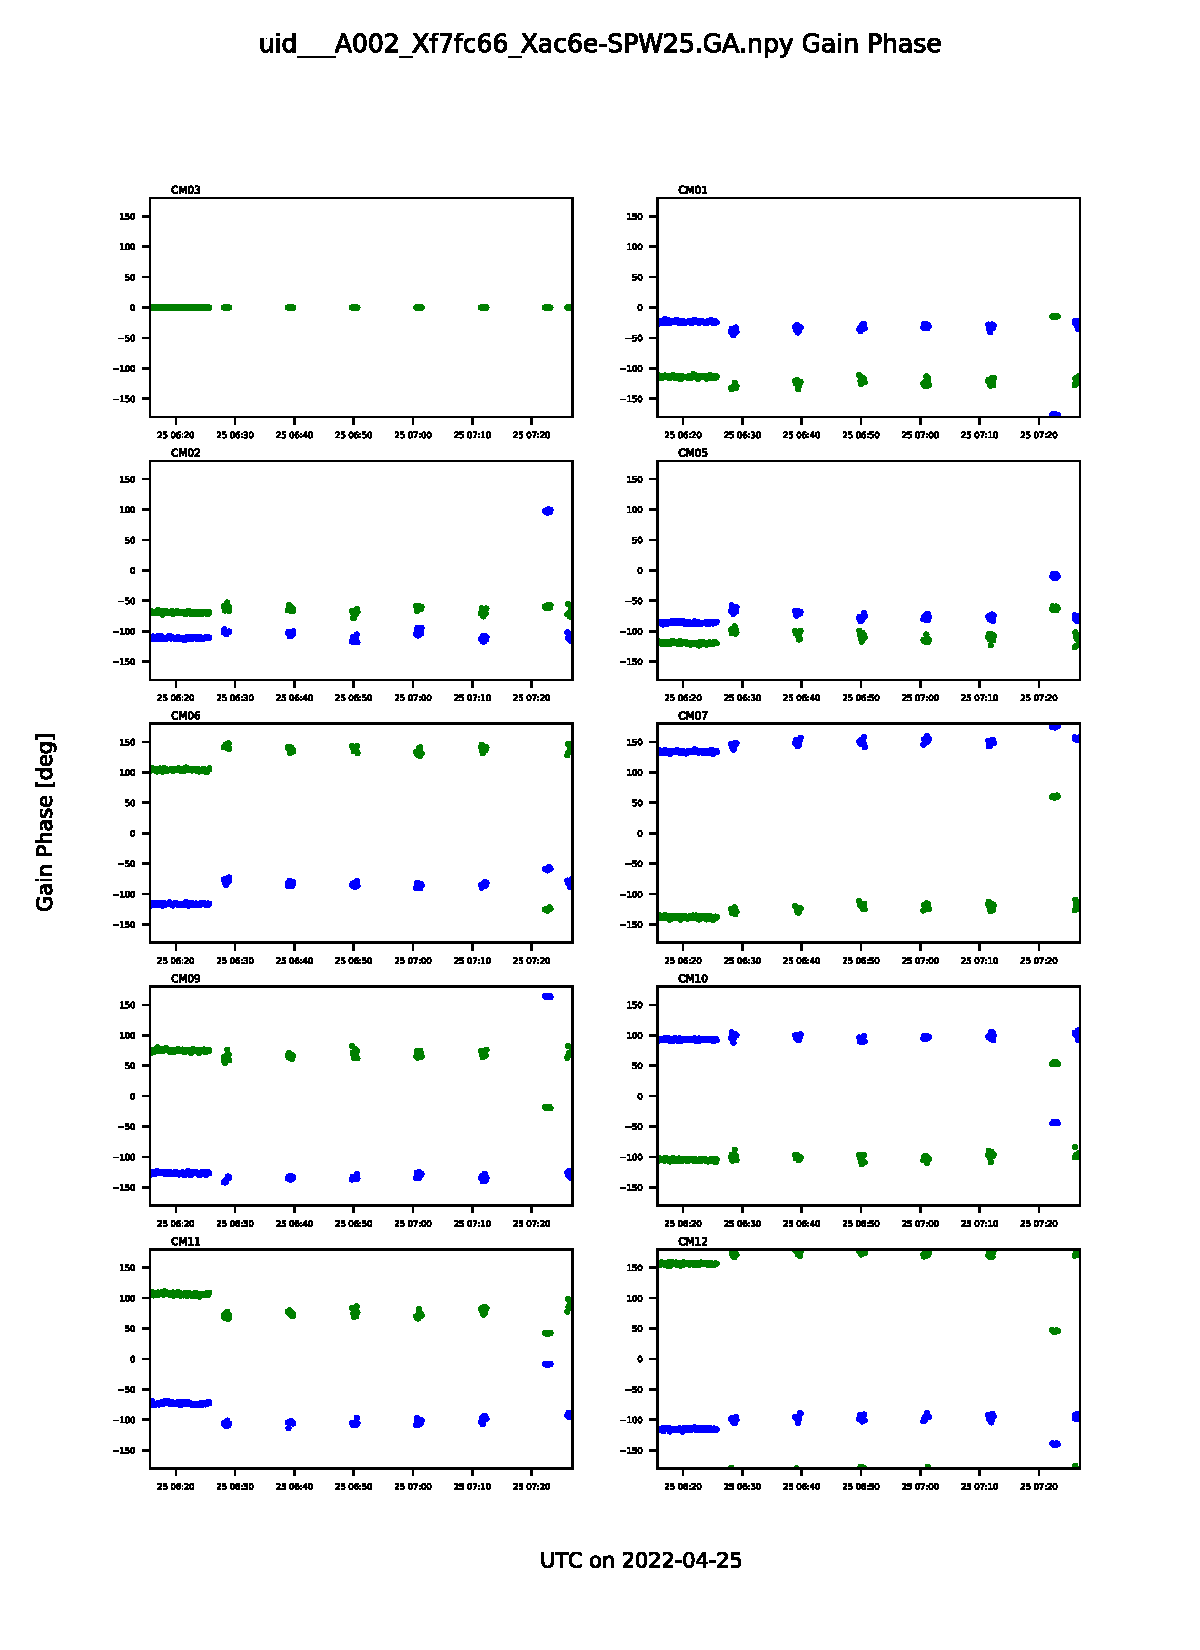
\includegraphics[width=7cm,height=6cm]{GA_uid___A002_Xf7fc66_Xac6e-SPW25-phs.pdf} 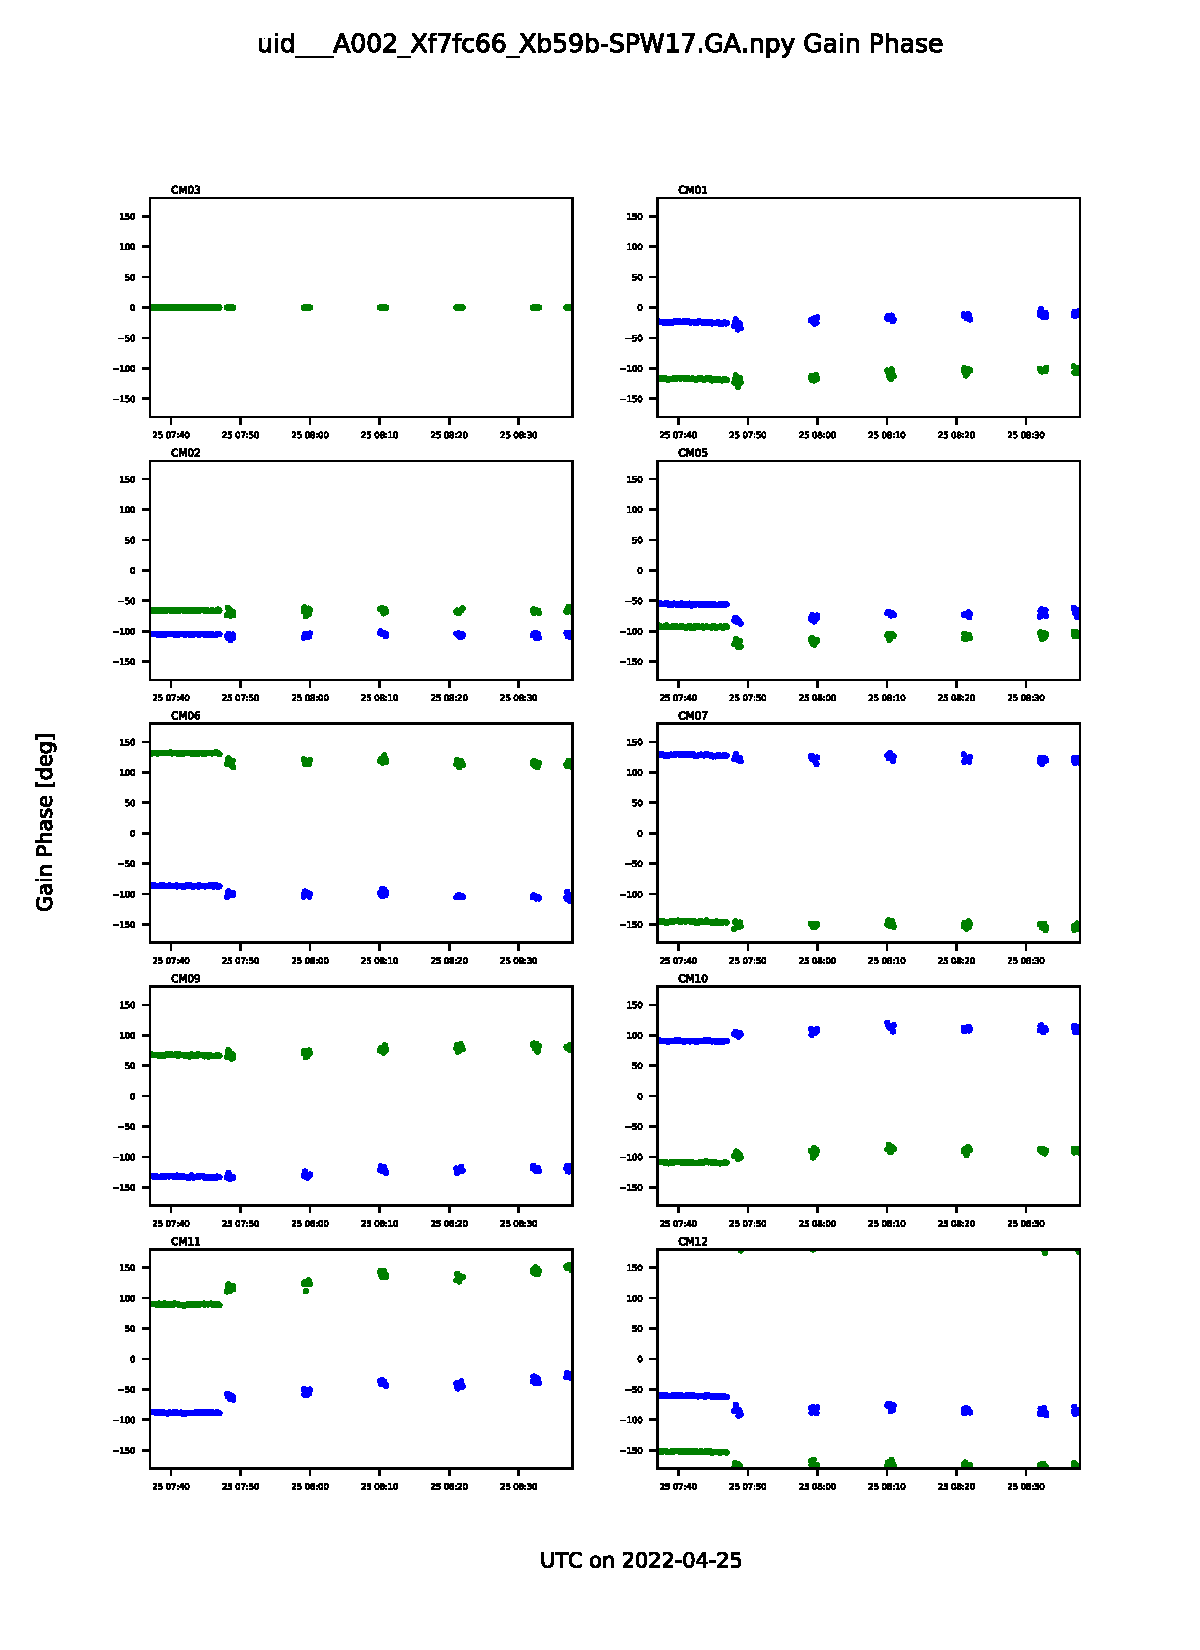
\includegraphics[width=7cm,height=6cm]{GA_uid___A002_Xf7fc66_Xb59b-SPW17-phs.pdf}
	\caption{Antenna-based gain amplitudes (Top) and phases (bottom) of spwID=0 (channel-averaged SPWs) in bandpass and phasecal scans in Xf7fc66/Xac6e (left) and Xf7fc66/Xb59b (right). Note that 07:21:15 -- 07:24:10 are unrealistic because of the anomalous cross correlations shown in figure \ref{fig:flagout}.}\label{fig:gainamp}
\end{figure}


\normalsize
\subsection{Spectral Setups}
The spectral setup are summarized in Table \ref{tab:SPW}. Scans for the target source consists of 2 narrow-band SPWS (SPW ID = 0, 1) with 937.5 MHz/3840 ch, and two TDM SPW (SPW ID=2, 3) with 2000 MHz/128 ch.
We used SPWID=0 for spectral line imaging and SPW=2,3 (combined) for continuum.
We didn't produced synthesis images in SPWID=1 targeting $^{13}$CO and C$^{18}$O which are too extended to produce interferometric images.

\begin{table}[h]
\centering
\caption{Spectral Setup}
\label{tab:SPW}
\begin{tabular}{l|rrrr} \hline \hline
SPW ID  &  0 &  1 &  2 &  3  \\
BB      &  1 &  2 &  3 &  4  \\
BLC SPW & 24 & 26 & 20 & 22  \\
ACAC SPW& 16 & 18 & 20 & 22  \\ 
Frequency (GHz)  &  218.518 & 220.019 & 233.020 & 235.020 \\
ChanWid (kHz)    & -244.141 & -488.281& 15625   & 15625 \\ 
Remarks &  H$_2$CO, CH$_3$OH & $^{13}$CO, C$^{18}$O & \multicolumn{2}{c}{continuum} \\ \hline
\end{tabular}
\end{table}

\section{Results}
\subsection{Phase Calibrator}\label{subsec:phasecal}

Continuum images of the phase calibrator, J1733-3722, were obtained in each SPW ID.
Flux density of the unresolved point-like component are listed in Table \ref{tab:contimage}.
The mean value of the ratio of flux densities correlated with BLC to ACA is 0.9989, indicating the difference in flux scaling $< 0.2$\%.

\begin{table}[h]
\centering
\caption{Parameters of the continuum maps. Columns (2): peak intensity near the northern edge, (3): integrated flux density obtained by Gaussian fit to the northern edge component (4): integrated flux density inside a 30-pixel circle centered at the source position.}
\label{tab:contimage}
\begin{tabular}{l|r|r|r|r} \hline \hline
SPW ID & 0      & 1      & 2  & 3  \\ \hline
BLC flux (Jy)   & 0.5093 & 0.5048 & 0.4910 & 0.4866 \\
ACAC flux (Jy)  & 0.5100 & 0.5059 & 0.4905 & 0.4874 \\ 
Ratio (BLC/ACAC)& 0.9985 & 0.9978 & 1.0010 & 0.9984 \\ \hline
\end{tabular}
\end{table}

Antenna-based gains of the phase calibrator are plotted in figure \ref{fig:gainamp}.
We used CM03 as the reference antenna and set solint=5 s for the plot.
To evaluate phase calibration performance in target scans sandwiched by phase calibrations scans, we obtained gain solutions with solint=60 s and obtained metrics summarized in Table \ref{tab:phasecal}. While phase rms is calculated by $\sqrt{ \left< (\phi_{k} - \bar{\phi})^2 \right> }$, phase difference is evaluated by $\left< | \phi_{k+1} - \phi_k  | \right>$, where $k$ stand for phase calibration scan index.

\begin{table}[h]
\centering
\caption{Phase metrics (degrees) in phase calibrator scans. Scan 26 in Xf7fc66/Xac6e is flagged out because of anomalous cross correlations.}
\label{tab:phasecal}
\begin{tabular}{l|rrrr|rrrr} \hline \hline
EB   & \multicolumn{4}{|c}{Xf7fc66/Xac6e} & \multicolumn{4}{|c}{Xf7fc66/Xb59b} \\
Metric & \multicolumn{2}{|c}{rms} & \multicolumn{2}{c}{diff} & \multicolumn{2}{|c}{rms} & \multicolumn{2}{c}{diff} \\
Pol.  & X & Y & X & Y & X & Y & X & Y \\ \hline
CM01 & 4$^{\circ}.$11 & 4$^{\circ}.$04 & 2$^{\circ}.$75 & 4$^{\circ}.$67 & 6$^{\circ}.$64 & 6$^{\circ}.$37 & 3$^{\circ}.$84 & 3$^{\circ}.$79 \\
CM02 & 4$^{\circ}.$76 & 3$^{\circ}.$60 & 8$^{\circ}.$45 & 6$^{\circ}.$13 & 1$^{\circ}.$45 & 0$^{\circ}.$98 & 1$^{\circ}.$62 & 1$^{\circ}.$31 \\
CM05 & 5$^{\circ}.$54 & 5$^{\circ}.$14 & 0$^{\circ}.$90 & 2$^{\circ}.$62 & 5$^{\circ}.$05 & 5$^{\circ}.$14 & 3$^{\circ}.$13 & 1$^{\circ}.$99 \\
CM06 & 2$^{\circ}.$39 & 2$^{\circ}.$99 & 2$^{\circ}.$22 & 5$^{\circ}.$15 & 2$^{\circ}.$69 & 2$^{\circ}.$66 & 0$^{\circ}.$63 & 1$^{\circ}.$03 \\
CM07 & 3$^{\circ}.$58 & 3$^{\circ}.$67 & 3$^{\circ}.$46 & 3$^{\circ}.$69 & 2$^{\circ}.$53 & 1$^{\circ}.$84 & 1$^{\circ}.$76 & 1$^{\circ}.$83 \\
CM09 & 3$^{\circ}.$39 & 2$^{\circ}.$69 & 4$^{\circ}.$00 & 1$^{\circ}.$95 & 5$^{\circ}.$34 & 5$^{\circ}.$21 & 2$^{\circ}.$37 & 2$^{\circ}.$32 \\
CM10 & 2$^{\circ}.$93 & 2$^{\circ}.$96 & 3$^{\circ}.$69 & 1$^{\circ}.$22 & 3$^{\circ}.$95 & 3$^{\circ}.$19 & 4$^{\circ}.$13 & 2$^{\circ}.$67 \\
CM11 & 5$^{\circ}.$19 & 5$^{\circ}.$80 & 2$^{\circ}.$09 & 5$^{\circ}.$57 & 11$^{\circ}.$6 & 11$^{\circ}.$6 & 7$^{\circ}.$95 & 6$^{\circ}.$65 \\
CM12 & 1$^{\circ}.$46 & 1$^{\circ}.$78 & 0$^{\circ}.$70 & 2$^{\circ}.$40 & 3$^{\circ}.$08 & 2$^{\circ}.$00 & 3$^{\circ}.$35 & 2$^{\circ}.$15 \\ \hline
\end{tabular}
\end{table}

Based on the phase metrics, we evaluate the coherence in taget scans by $\exp \left( -\frac{\phi^2_{rms} }{2} \right)$, and got 0.998 and 0.995 for BLC and ACAC, respectively.

\subsection{Target continuum images}\label{subsec:contimages}
We used tclean() with a mask
circle[[164pix,98pix],10pix] 
to produce the continuum images combining SPW ID=2 and 3.
A common circular restring beam of $8^{\prime \prime}$ is employed for both images.
Figure \ref{fig:contimage} shows the continuum images of ClusterC obtained by BLC and ACAC, respectively. We detected a slightly resolved feature centered at $17^h 00^m 32^s.47$, $-40^{\circ} 34^{\prime} 9^{\prime \prime}.0$.

Continuum peak intensities and flux densities inside a 10-pixel circle centered at $17^h 00^m 32^s.47$, $-40^{\circ} 34^{\prime} 9^{\prime \prime}.0$ are listed in table \ref{tab:contimage}.

\begin{figure}[h]
	\centering
	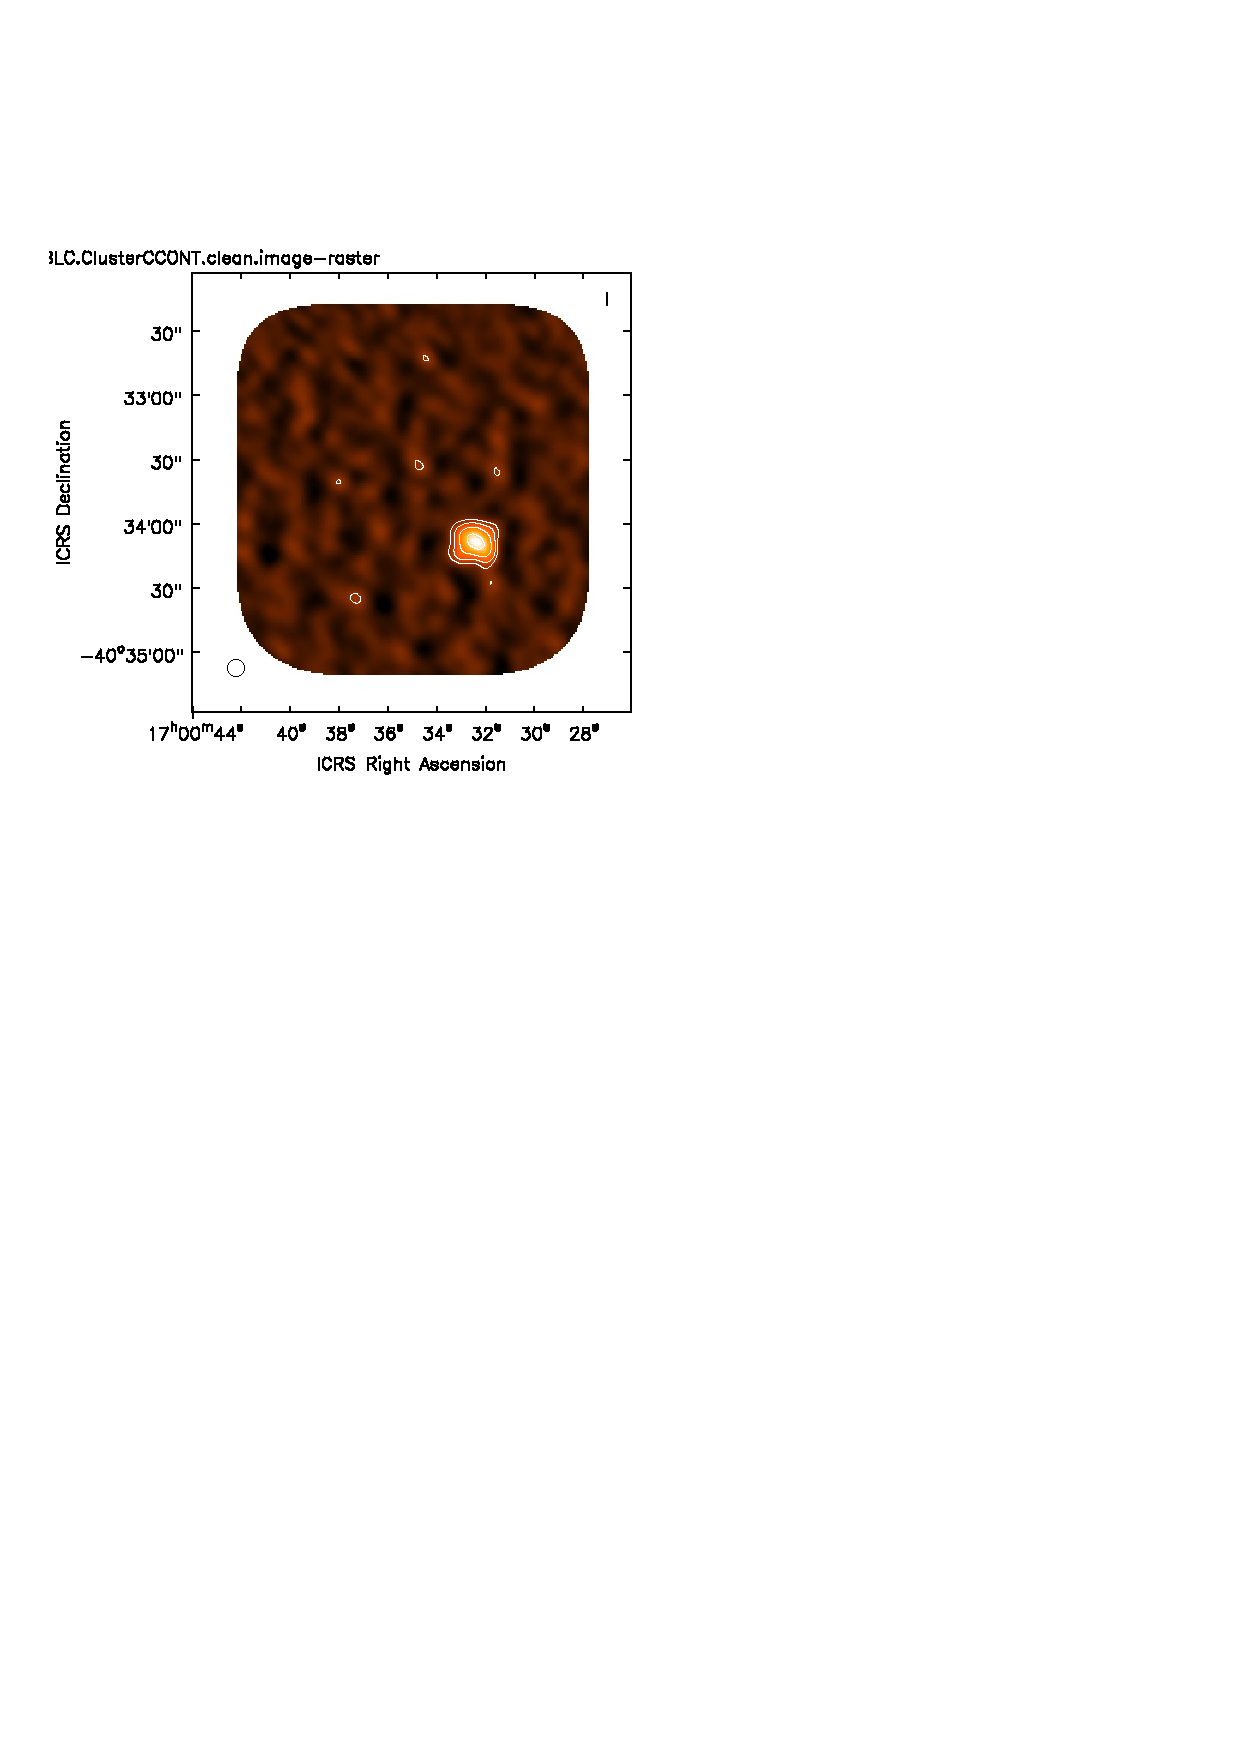
\includegraphics[width=7.5cm]{BLC.ClusterC.pdf}
	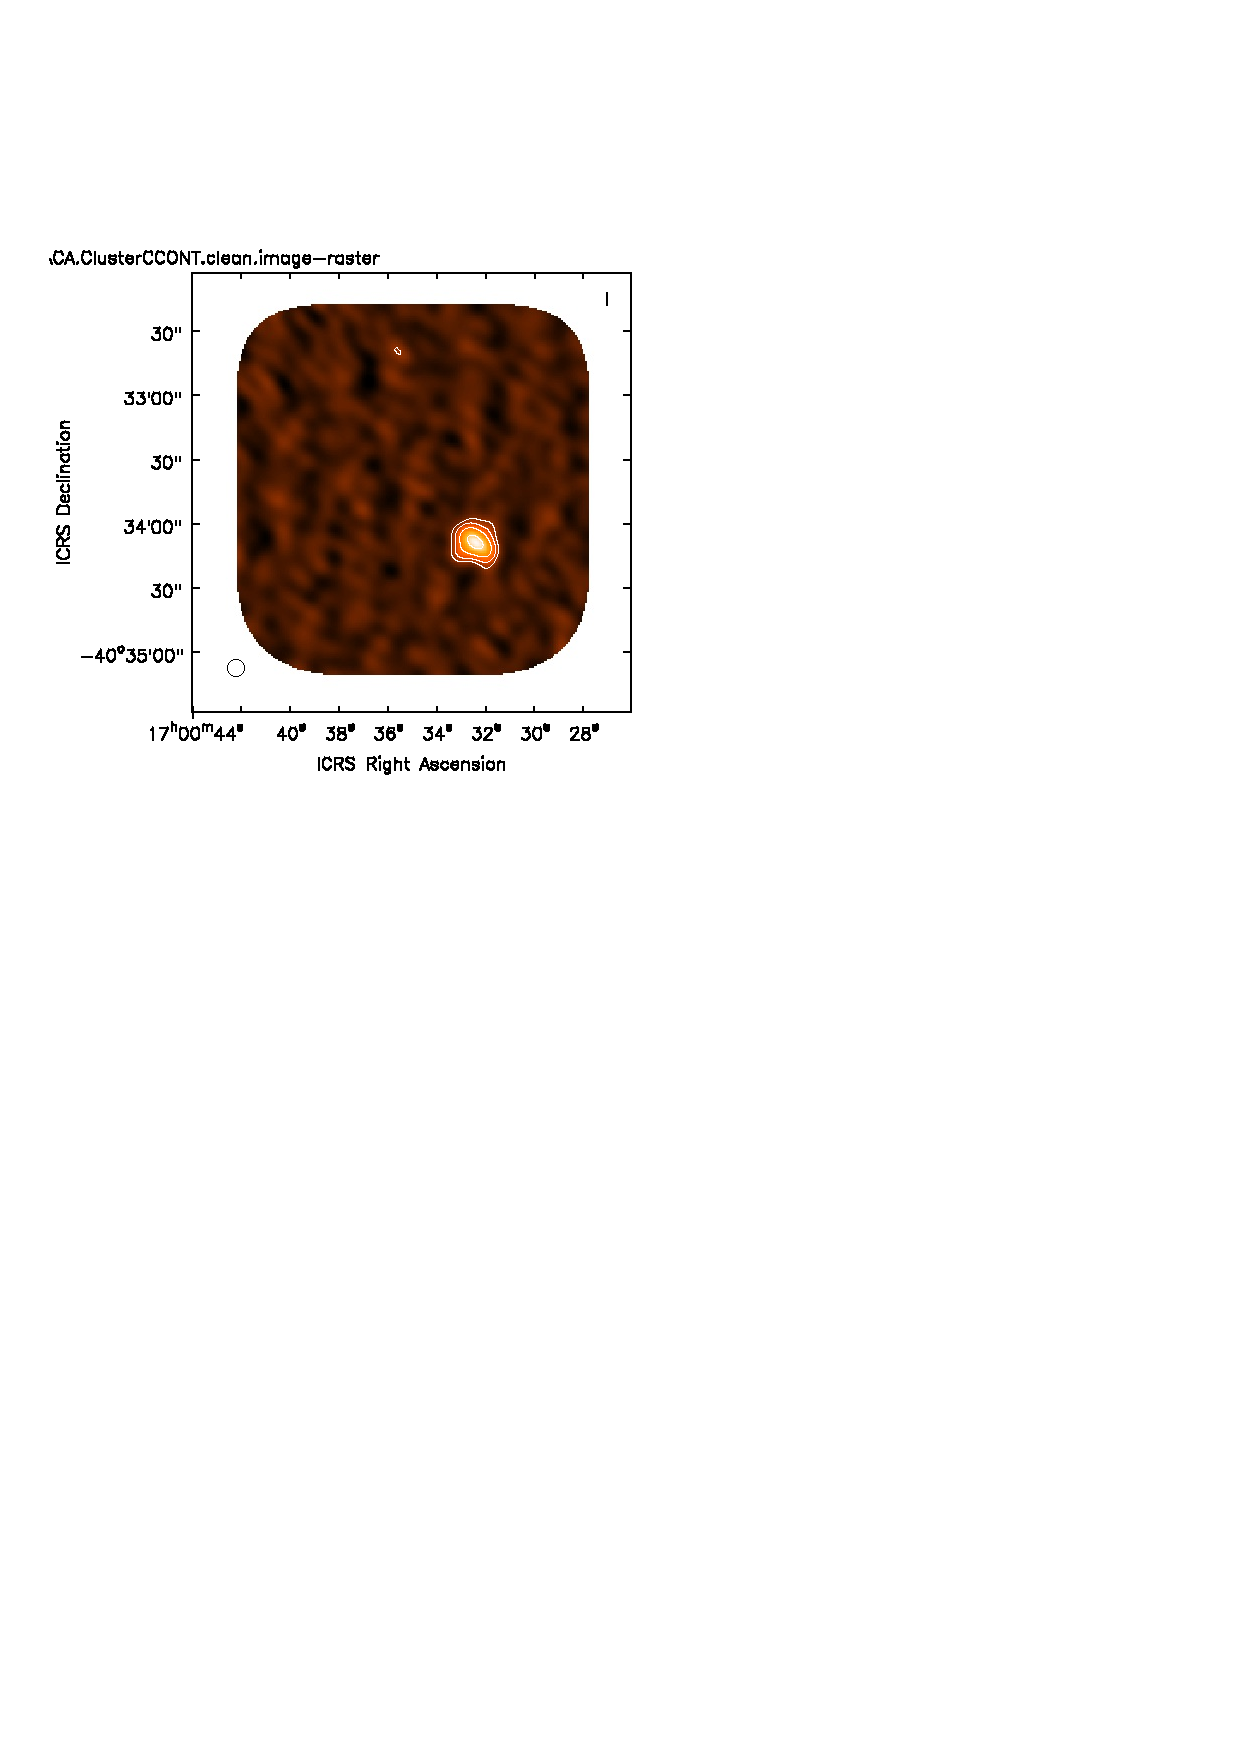
\includegraphics[width=7.5cm]{ACA.ClusterC.pdf}
	\caption{CLEANed continuum images of ClusterC correlated with BLC (left) and ACAC (right). Contour levels are $(1, 2, 4, 8) \times 1$ mJy/beam.}\label{fig:contimage}
\end{figure}

\begin{table}[h]
\centering
\caption{Parameters of the continuum maps. Columns (2): peak intensity near the northern edge, (3): integrated flux density obtained by Gaussian fit to the northern edge component (4): integrated flux density inside a 10-pixel circle centered at $17^h 00^m 32^s.47$, $-40^{\circ} 34^{\prime} 9^{\prime \prime}.0$ }
\label{tab:contimage}
\begin{tabular}{l|r|r|r} \hline \hline
Corr.  & Peak Intensity   & Flux density  & Image rms\\
       & (mJy/beam)       & (mJy)         & (mJy/beam) \\ \hline
BLC    & 100.91           & 244.2         & 3.55   \\
ACAC   &  96.62           & 222.9         & 3.54   \\ 
Ratio (BLC/ACAC) & 1.044  & 1.096         & -          \\ \hline
\end{tabular}
\end{table}

Unlike the phase calibrator, continuum flux densities of the target, ClusterC, is slightly different between BLC and ACAC.

\subsection{Spectral lines}\label{subsec:lineimages}
Channel map of the strongest emission line, H$_2$CO 3(0,3)-2(0,2), are presented in figure \ref{fig:H2COchanMap}. For the channel map, no artificial restoring beam was employed. CLEAN boxes are interactively set for each channel. The channel maps demonstrates complex structure of the source.  

\begin{figure}[h]
	\centering
	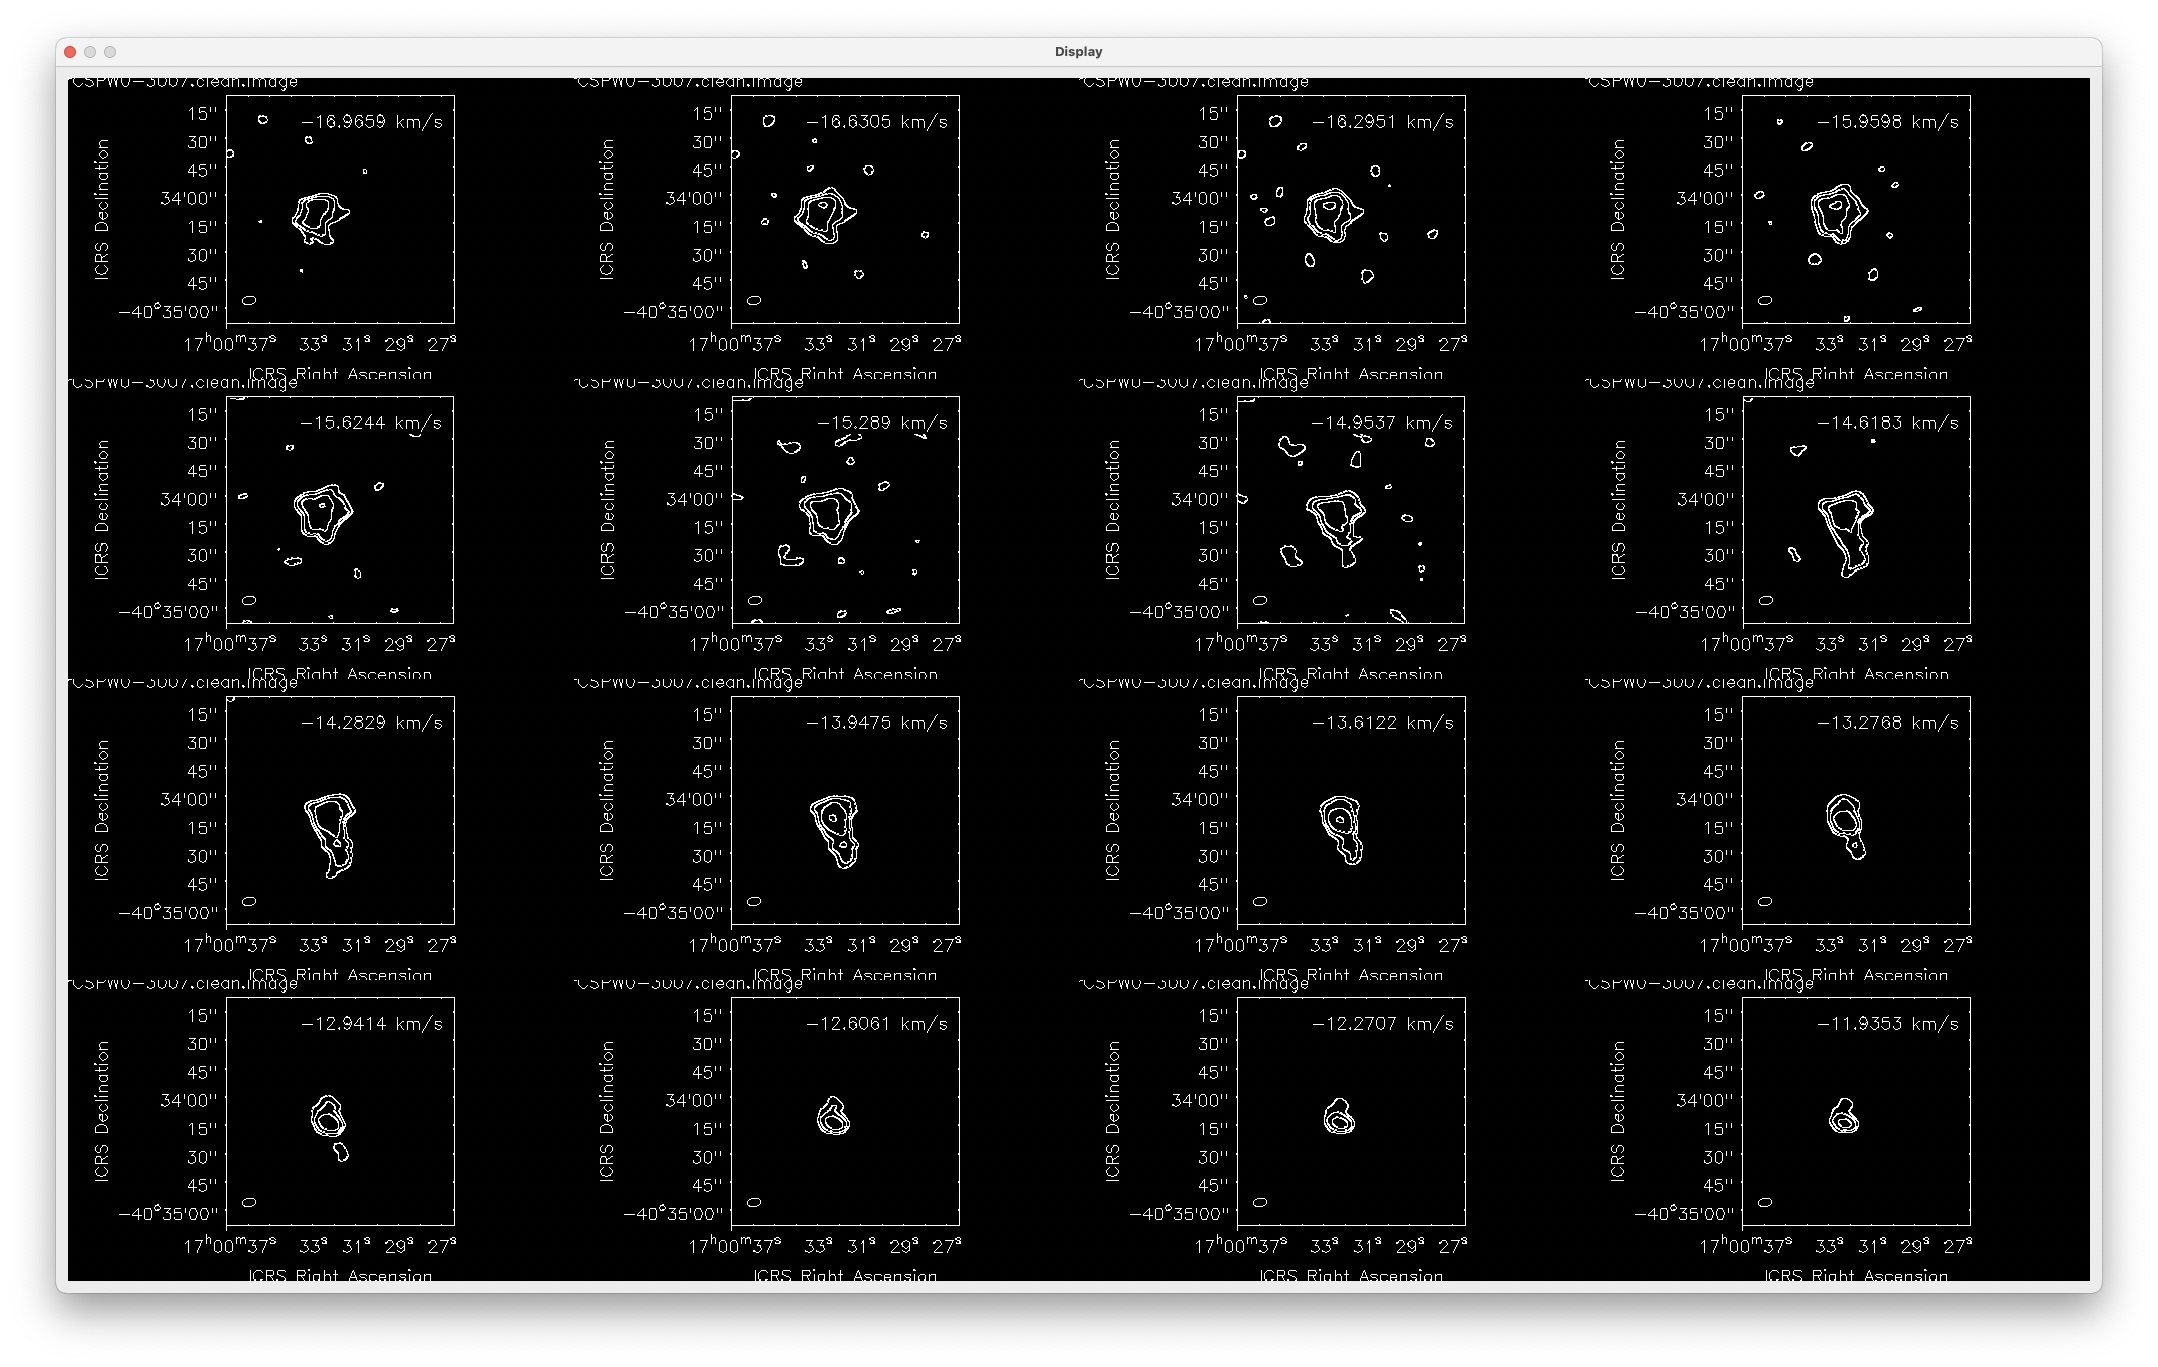
\includegraphics[width=15cm]{BLC-ChanMap.png}
	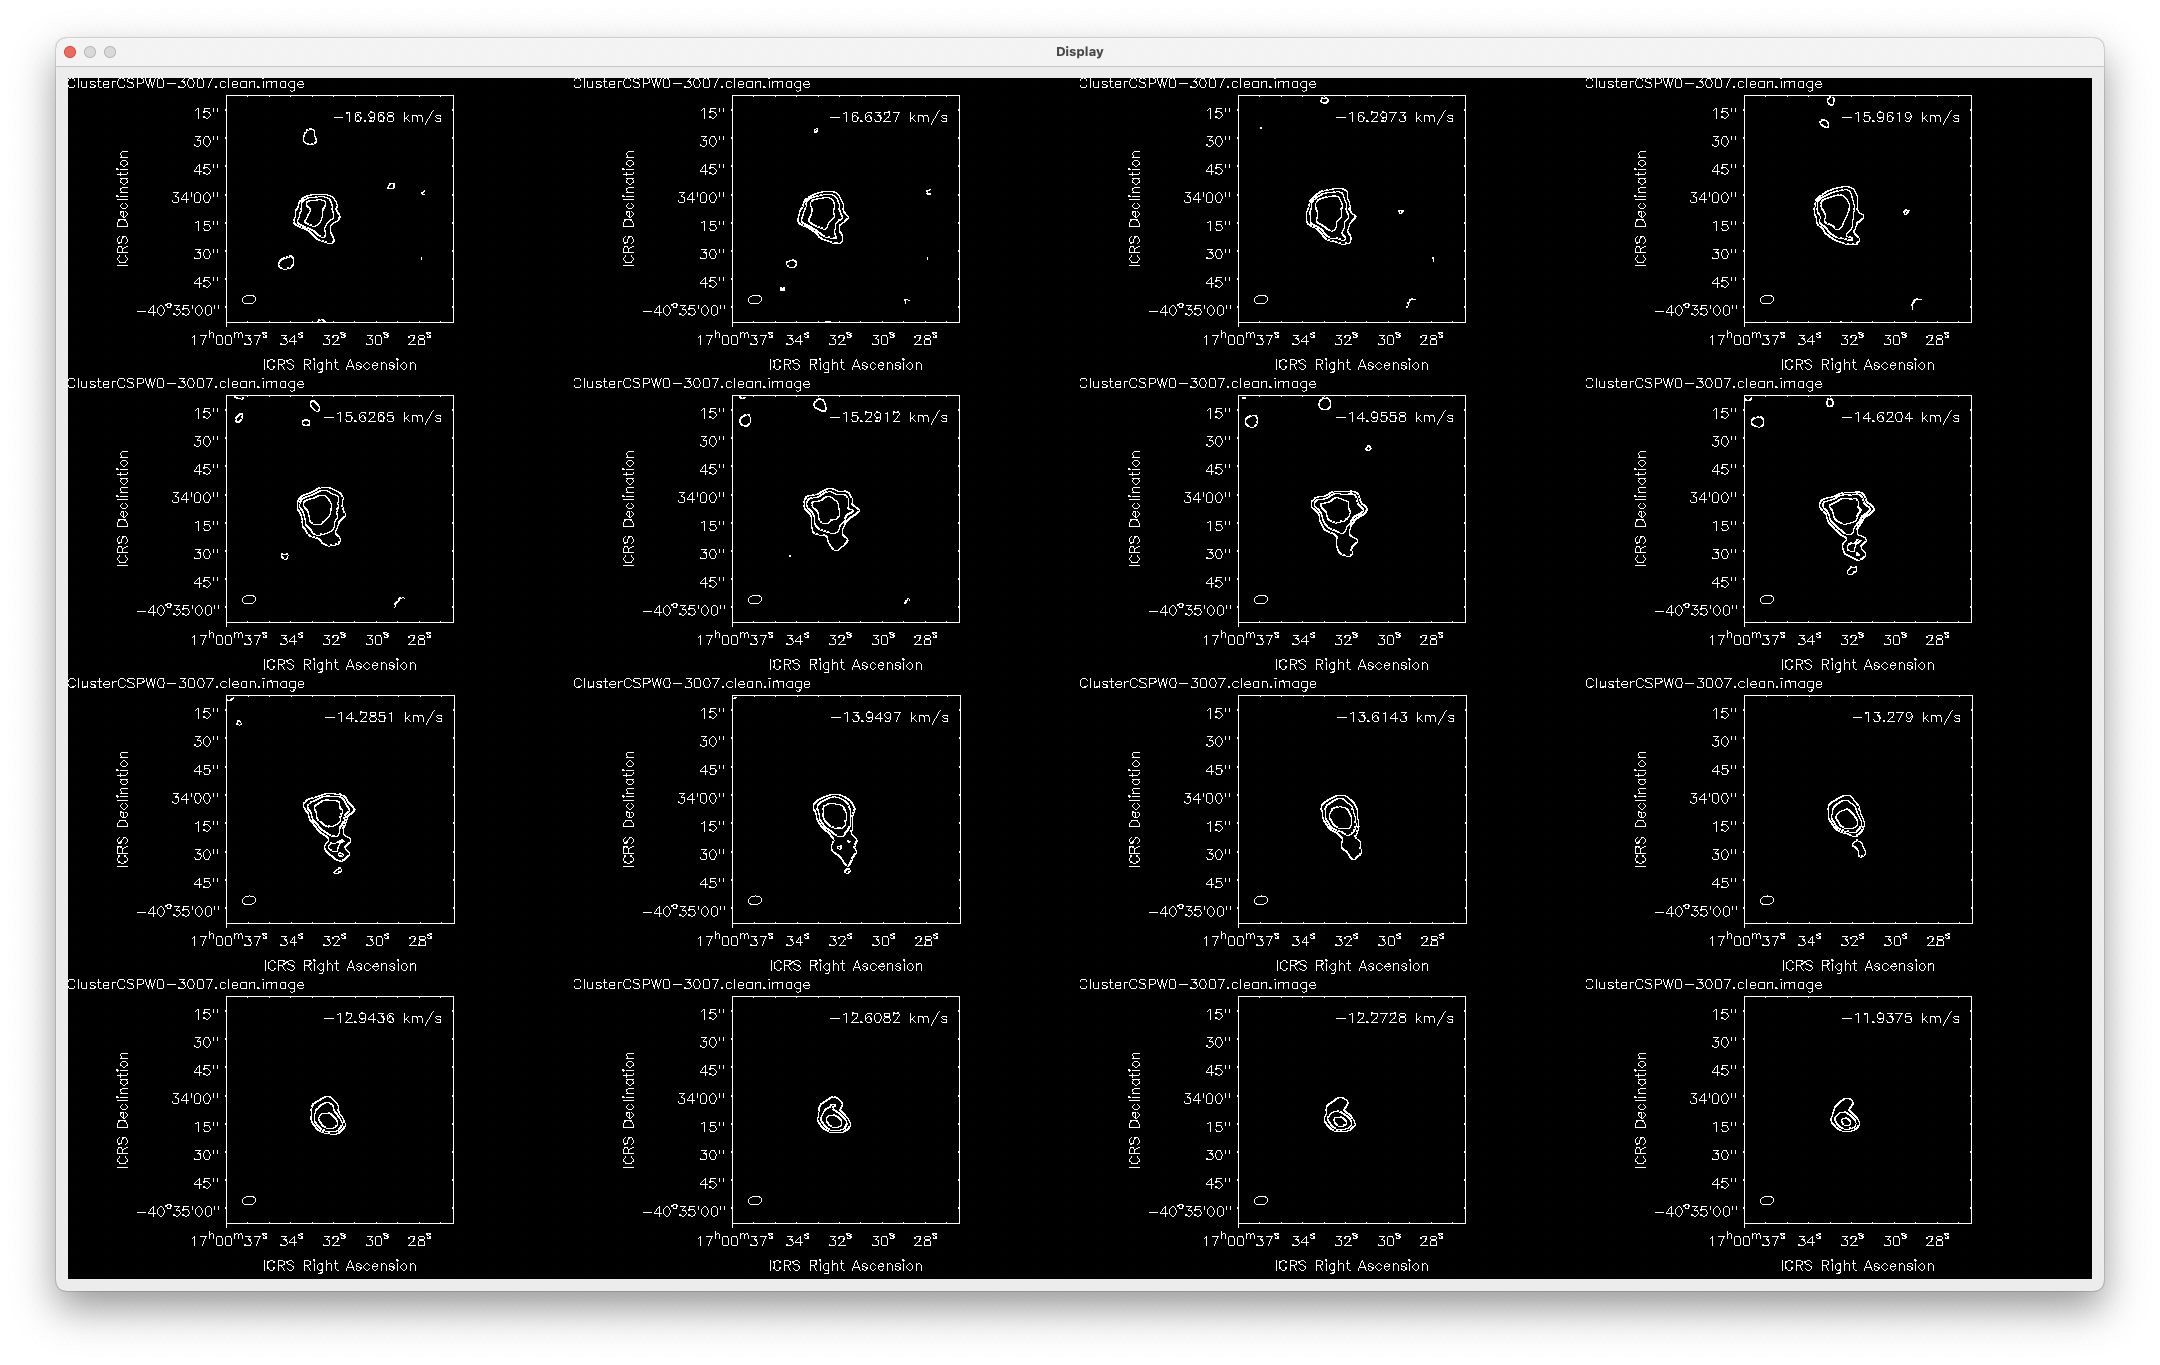
\includegraphics[width=15cm]{ACA-ChanMap.png}
	\caption{Channel maps of H$_2$CO 3(0,3)-2(0,2) correlated with BLC (left) and ACAC (right). Contour levels are at (0.1, 0.2, 0.4, 0.8, 1.6,  3.2) Jy/beam. The channel maps didn't employ any artificial restoring beam. CLEAN boxes are interactively set to avoid negative brightness.}\label{fig:H2COchanMap}
\end{figure}

To evaluate spectral line profiles, we generated image cubes were in SPW ID = 0, which includes three H$_2$CO transitions and one CH$_3$OH emission.
We used the same mask of circle[[164pix,98pix],10pix] and the same restoring beam of $8^{\prime \prime}$ for producing image cubes.
Figure \ref{fig:SPW0} shows the overall spectra of SPW ID=0 containing H$_2$CO 3(0,3)-2(0,2), H$_2$CO 3(2,2)-2(2,1), H$_2$CO 3(2,1)-2(2,0), and CH$_3$OH 4(2) - 3(1) transitions at the rest frequencies of 218.22219 GHz, 218.475632 GHz, 218.760066 GHz, and 218.44006 GHz, respectively.

\begin{figure}[h]
	\centering
	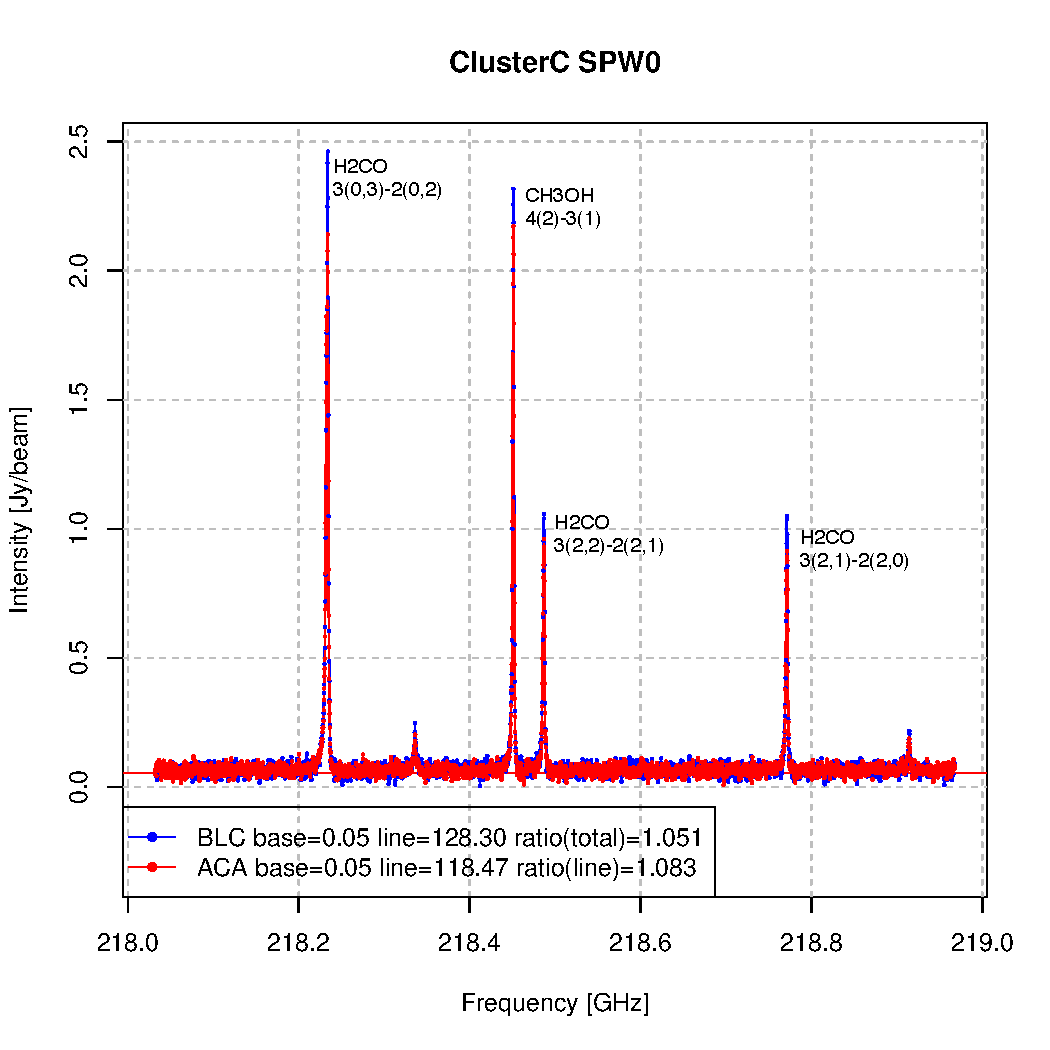
\includegraphics[width=10cm]{ClusterC.SPW0.pdf}
	\caption{Whole spectra of SPW ID = 0 obtained by BLC (blue) and ACAC (red). Four outstanding features stand for H$_2$CO 3(0,3)-2(0,2), H$_2$CO 3(2,2)-2(2,1), H$_2$CO 3(2,1)-2(2,0), and CH$_3$OH 4(2) - 3(1) transitions at the rest frequencies of 218.22219 GHz, 218.475632 GHz, 218.760066 GHz, and 218.44006 GHz, respectively.}\label{fig:SPW0}
\end{figure}

Figure \ref{fig:H2COimageSpec} shows the peak channel maps of H$_2$CO 3(2,2)-3(2,1) and integrated spectra inside a 10-pixel circle centered at $17^h 00^m 32^s.47$, $-40^{\circ} 34^{\prime} 9^{\prime \prime}.0$.
Hot-metal raster and contours stand for the peak channel map correlated by BLC and ACAC, respectively.
The integral region is indicated by a pink circle in the peak channel map.

\begin{figure}[h]
	\centering
	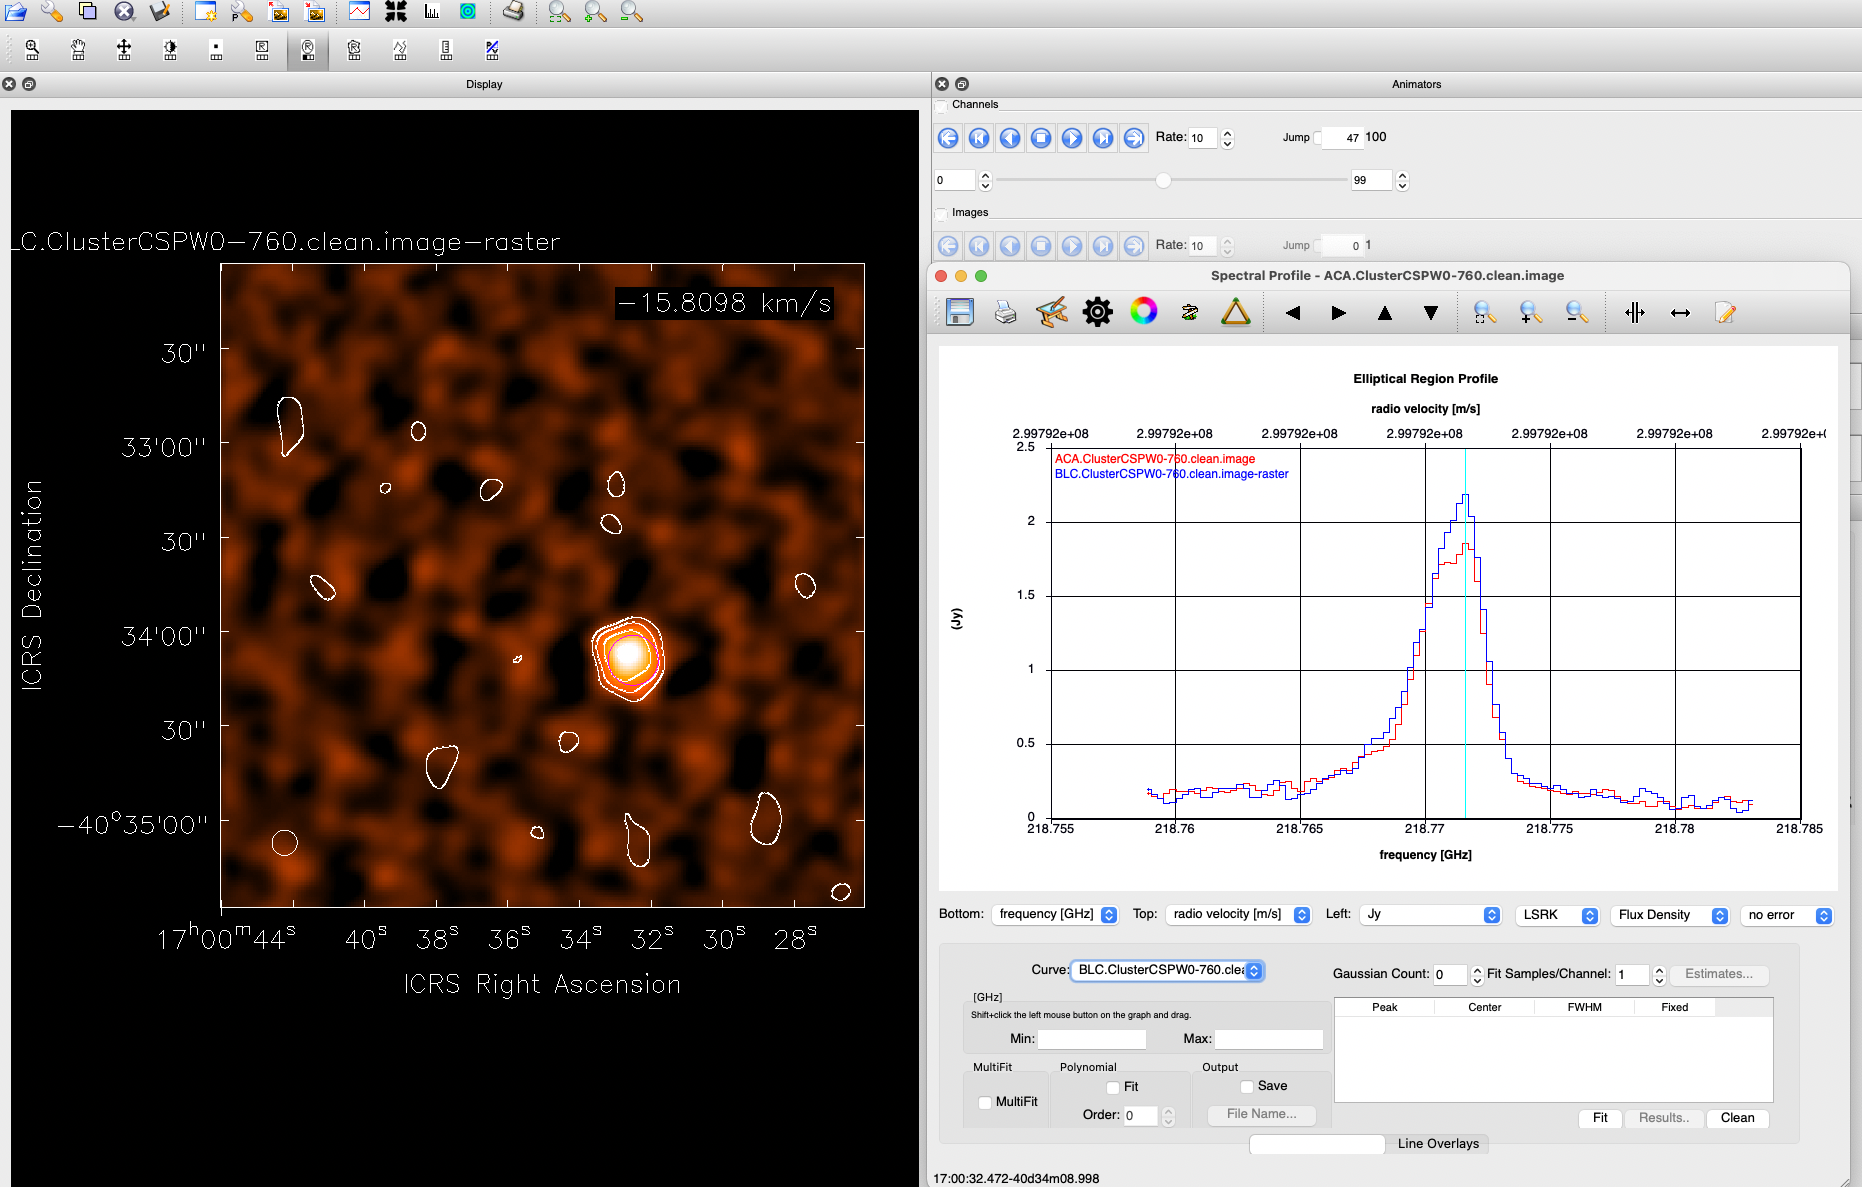
\includegraphics[width=12cm]{ClusterC-SPW0.png}
	\caption{H$_2$CO channel map of ClusterC correlated with BLC (hot-metal raster map) and ACAC (contour). Integrated spectra inside the purple circle are shown in the right panel.}\label{fig:H2COimageSpec}
\end{figure}

Figure \ref{fig:H2CO} displays spectra of individual line species integrated inside the circle shown in figure \ref{fig:H2COimageSpec}.
Blue and red lines stand for the spectra processed with BLC and ACAC, respectively.
Spectral channel misalignment between two ExecBlocks was 0.244141 ch. Thus, we applied spline smoothing and resampling to align the channelization.

\begin{figure}[h]
	\centering
	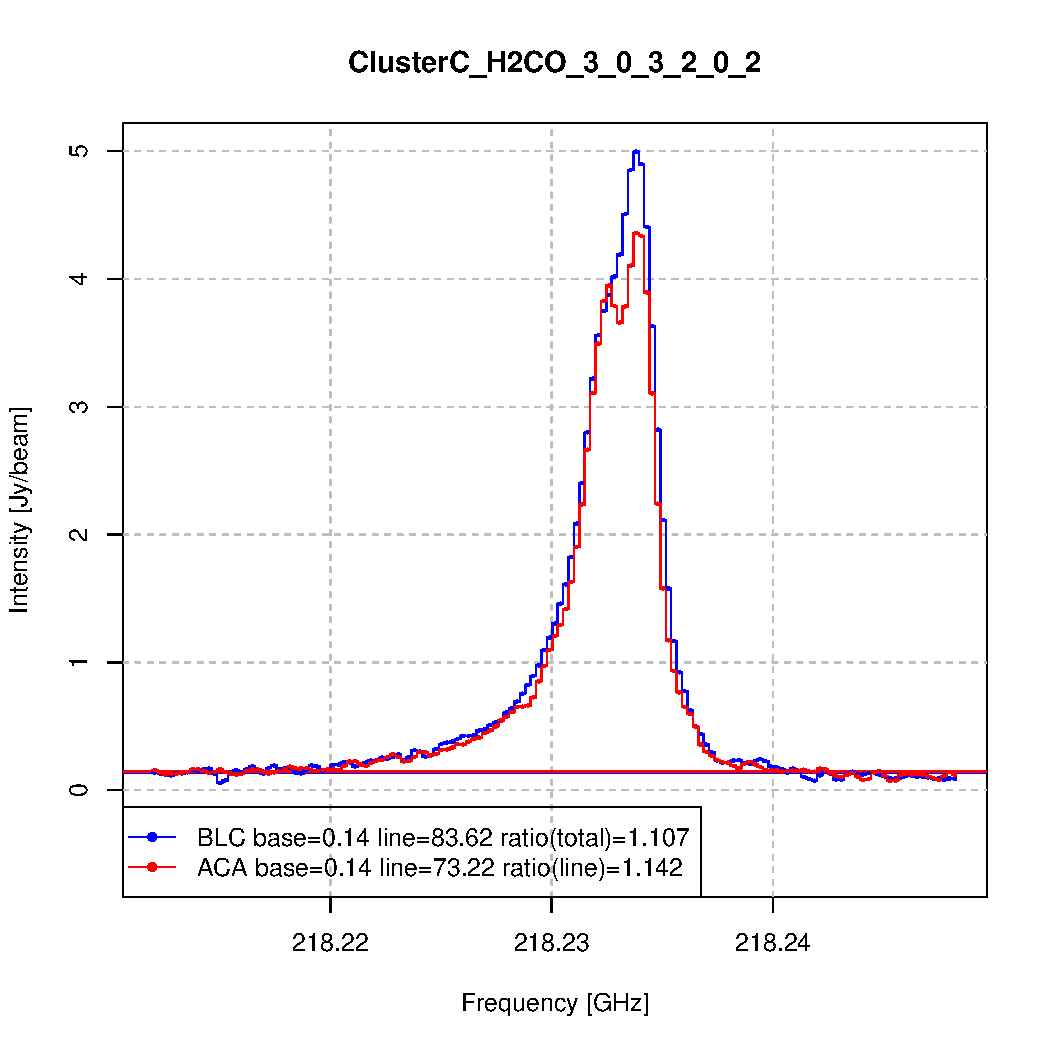
\includegraphics[width=7cm]{ClusterC_H2CO_3_0_3_2_0_2.pdf}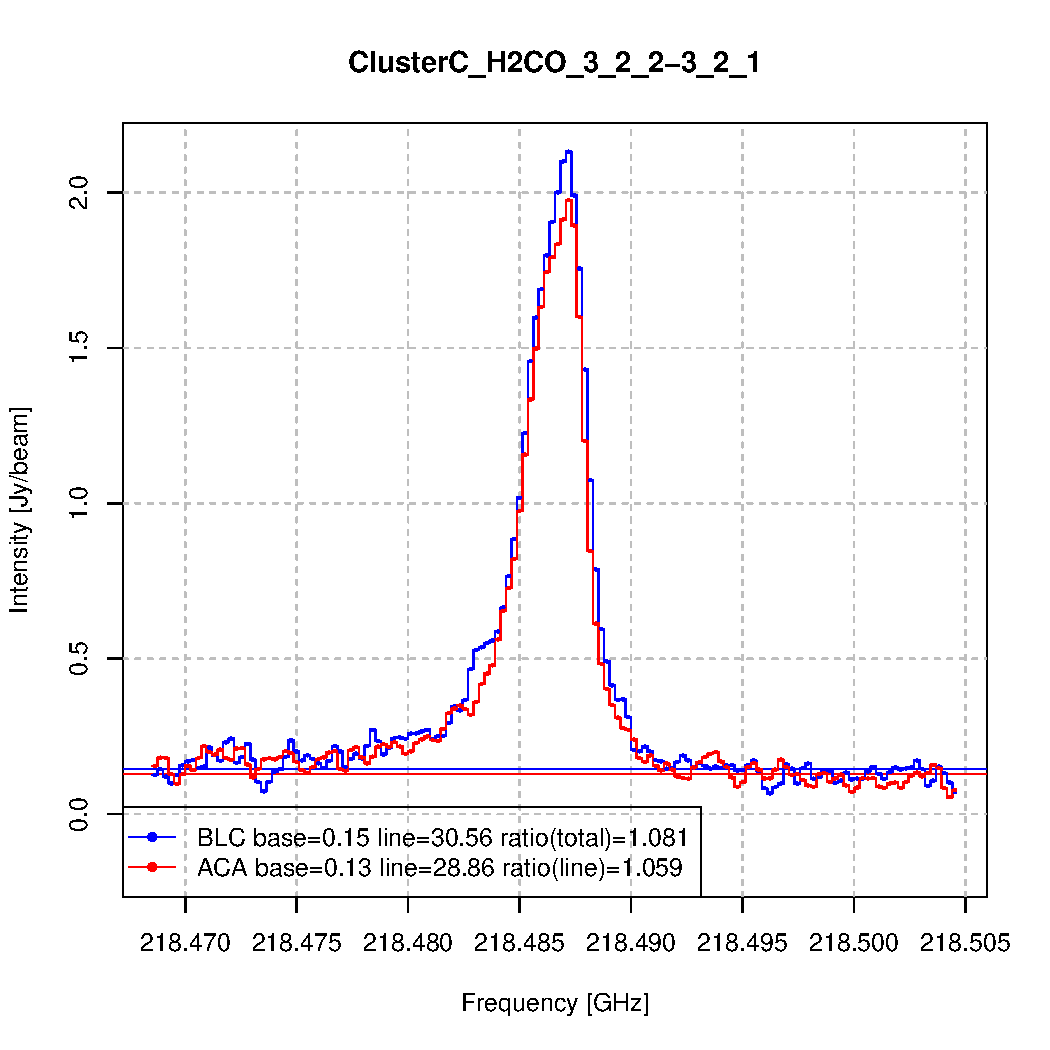
\includegraphics[width=7cm]{ClusterC_H2CO_3_2_2-3_2_1.pdf}
	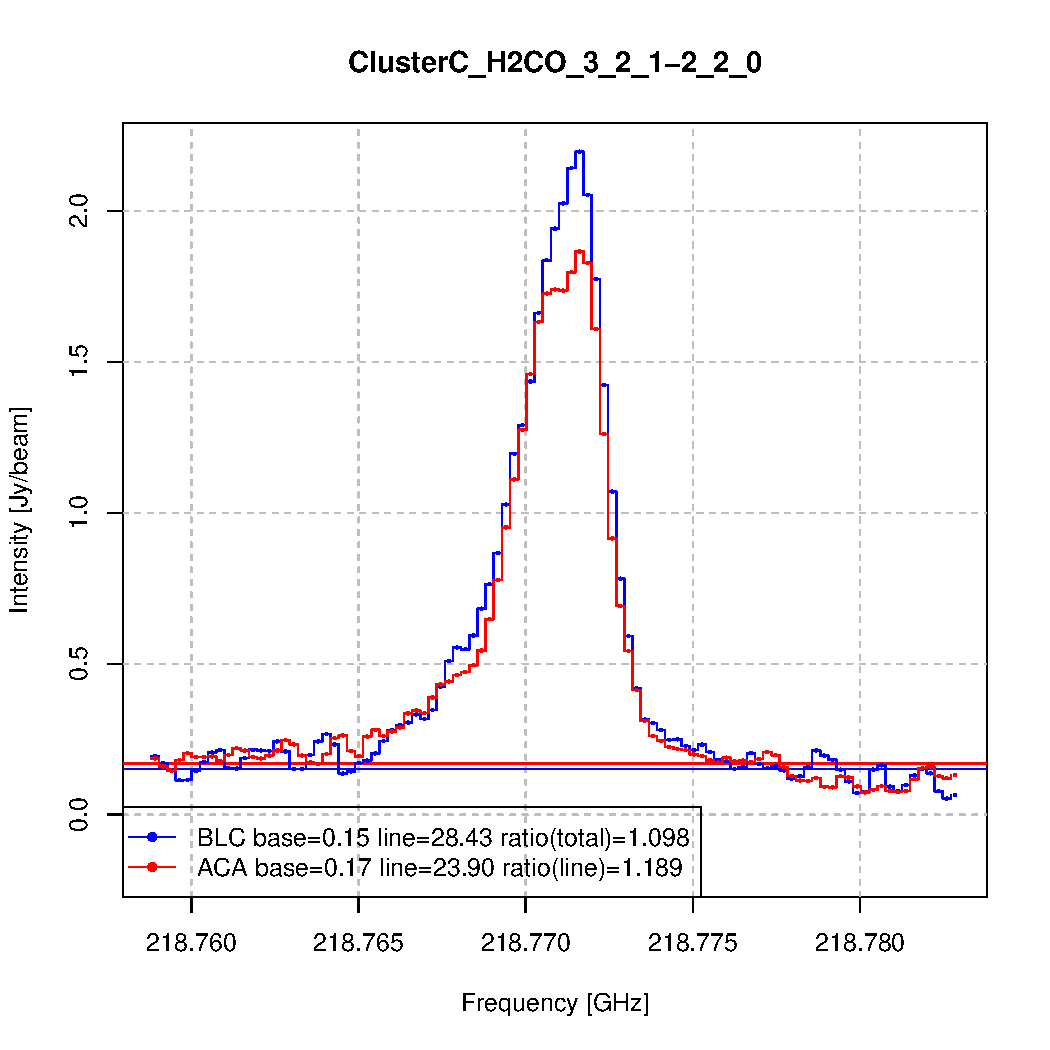
\includegraphics[width=7cm]{ClusterC_H2CO_3_2_1-2_2_0.pdf}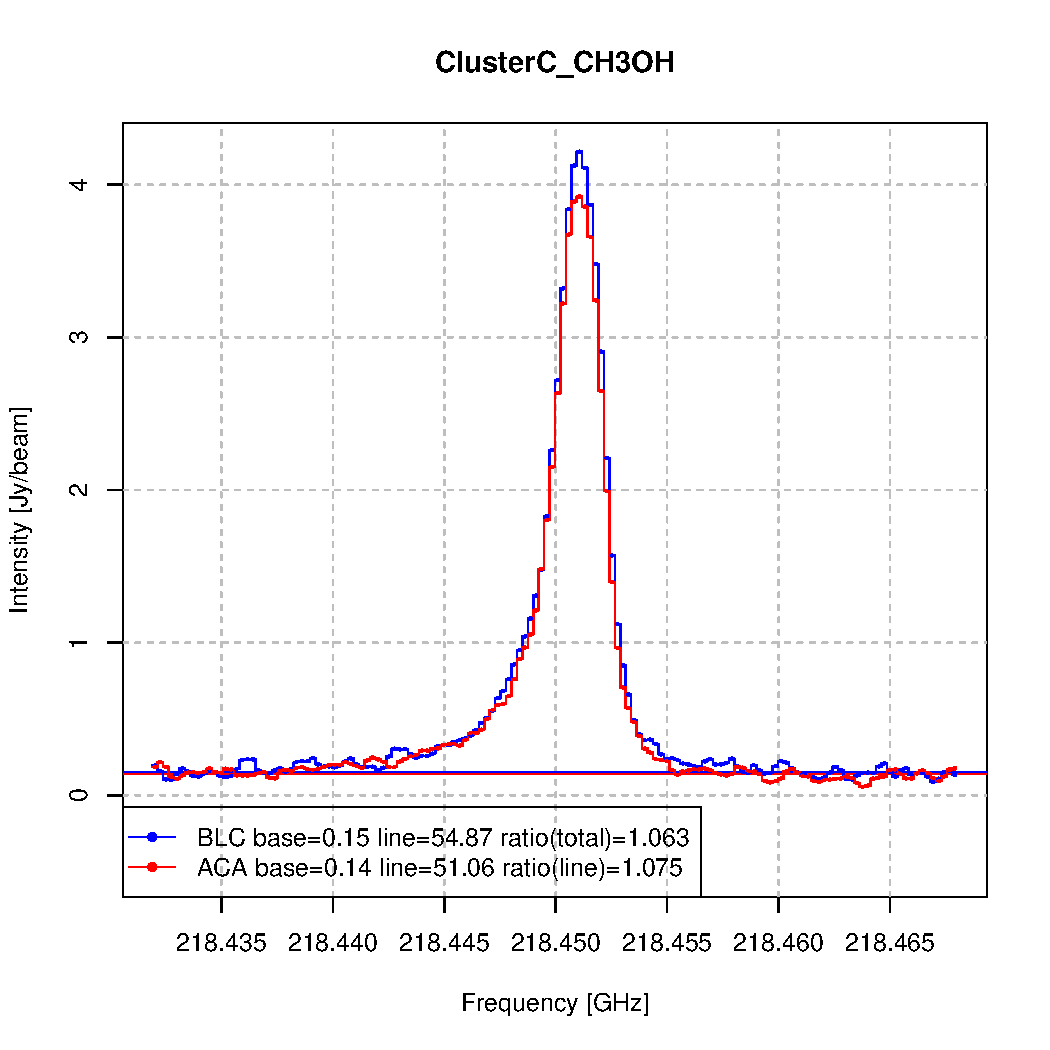
\includegraphics[width=7cm]{ClusterC_CH3OH.pdf}
	\caption{Integrated spectra. (Top left) H$_2$CO 3(0,3)-2(0,2), $\nu_{rest} = 218.22219$ GHz. (Top right) H$_2$CO 3(2,2)-2(2,1), $\nu_{rest} = 218.475632$ GHz. (Bottom left) H$_2$CO 3(2,1)-2(2,0), $\nu_{rest} = 218.760066$ GHz, and CH$_3$OH 4(2) - 3(1), $\nu_{rest} = 218.44006$ GHz.}\label{fig:H2CO}
\end{figure}


We have compared the spectra taken with BLC and ACAC by two measures.

\begin{itemize}
\item Total intensity ratio, $R$, obtained by \[ I^\mathrm{BLC}_{\nu} \sim R \cdot I^\mathrm{ACA}_{\nu}, \] where $\sim$ indicates linear regression without intercept.

\item Line flux ratio, $L$, obtained by \[ L = \frac{\sum_{\nu} (I^\mathrm{BLC}_{\nu} - B^\mathrm{BLC}_{\nu})}{\sum_{\nu} (I^\mathrm{ACA}_{\nu} - B^\mathrm{ACA}_{\nu}) }, \] where $B$ is a baseline level shown in the horizontal line in figure \ref{fig:SPW0}. The baseline level was determined by percentile of 40\% unless the spectral peak exceeds $2\times$ as high as the median, or 25\% percentile otherwise.
\end{itemize}

These two measures are listed in columns 3 and 4 in table \ref{tab:Spectra}.

\begin{table}[h]
\centering
\caption{Comparison of spectral features}
\label{tab:Spectra}
\begin{tabular}{lrrr} \hline \hline
Line        &  Diff. (ch)& Intensity Ratio & Line Ratio \\ \hline 
H$_2$CO 3(0,3)-2(0,2)  &  0.244141  & 1.107           & 1.142 \\
H$_2$CO 3(2,2)-2(2,1)  &  0.244141  & 1.081           & 1.059 \\
H$_2$CO 3(2,1)-2(2,0)  &  0.244141  & 1.098           & 1.189 \\
CH$_3$OH 4(2) - 3(1)   &  0.244141  & 1.063           & 1.075 \\ \hline
mean                   &            & 1.087           & 1.116 \\ \hline
\end{tabular}
\end{table}

\section{Discussion and Summary}
While flux densities of the phase calibrator, J1733-3722, were very consistent between BLC and ACAC, flux densities of continuum and emission lines in the target, ClusterC, were significantly different.
Integrated flux density of the target continuum measured by BLC is 9.6\% as high as that measured by ACAC.
The emission line intensities measured by BLC were also higher by 8.7\% (intensity ratio) or 11.6\% (line ratio) compared with ACAC.

Coherence loss in the target scans hardly accounts for the difference. The phase metrics listed in table \ref{tab:phasecal} indicates that coherence losses in target scans are estimated as 0.998 and 0.995 for BLC and ACAC, respectively (see section \ref{subsec:phasecal}).

It is notable that the target source has a resolved structure and the synthesized beams are different between two executions in terms of the position angle of the relatively high sidelobes.
Differences in responses to the extended structure by different synthesized beam woud cause the difference in continuum flux and line profiles. Note that the line-to-continuum ratios remain consistent between two correlators.

\end{document}
